\documentclass[a4paper]{report}
\usepackage[a4paper, margin=1.3in]{geometry}
% basics
\usepackage{siunitx}

\usepackage[utf8]{inputenc}
% \usepackage[swedish]{babel}
\usepackage{lmodern}
\usepackage[T1]{fontenc}
\usepackage[babel=true]{microtype}

\usepackage{url}
\usepackage{hyperref}
\hypersetup{
    colorlinks,
    linkcolor={blue},
    citecolor={black},
    urlcolor={blue!80!black}
}
\usepackage{graphicx}
\usepackage{float}
\usepackage{booktabs}
\usepackage{enumitem}
% \usepackage{parskip}
\usepackage{emptypage}
\usepackage{subcaption}
\usepackage{multicol}
\usepackage[usenames,dvipsnames]{xcolor}

% \usepackage{cmbright}


\usepackage{amsmath, amsfonts, mathtools, amsthm, amssymb}
\usepackage{mathrsfs}
\usepackage{cancel}
\usepackage{bm}
\newcommand\N{\ensuremath{\mathbb{N}}}
\newcommand\R{\ensuremath{\mathbb{R}}}
\newcommand\Z{\ensuremath{\mathbb{Z}}}
\renewcommand\O{\ensuremath{\emptyset}}
\newcommand\Q{\ensuremath{\mathbb{Q}}}
\newcommand\C{\ensuremath{\mathbb{C}}}
% \newcommand\.{\ensuremath{\cdot}}
\newcommand\znz{\ensuremath{\mathbb{Z}/n\mathbb{Z}}}

\DeclareMathOperator{\sgn}{sgn}
\usepackage{systeme}
\let\svlim\lim\def\lim{\svlim\limits}
\let\implies\Rightarrow
\let\impliedby\Leftarrow
\let\iff\Leftrightarrow
\let\epsilon\varepsilon
\usepackage{stmaryrd} % for \lightning
\newcommand\contra{\scalebox{1.1}{$\lightning$}}
% \let\phi\varphi





% correct
\definecolor{correct}{HTML}{009900}
\newcommand\correct[2]{\ensuremath{\:}{\color{red}{#1}}\ensuremath{\to }{\color{correct}{#2}}\ensuremath{\:}}
\newcommand\green[1]{{\color{correct}{#1}}}



% horizontal rule
\newcommand\hr{
    \noindent\rule[0.5ex]{\linewidth}{0.5pt}
}


% hide parts
\newcommand\hide[1]{}



% si unitx
\usepackage{siunitx}
\sisetup{locale = FR}
% \renewcommand\vec[1]{\mathbf{#1}}
\newcommand\mat[1]{\mathbf{#1}}


% tikz
\usepackage{tikz}
\usepackage{tikz-cd}
\usetikzlibrary{intersections, angles, quotes, calc, positioning}
\usetikzlibrary{arrows.meta}
\usepackage{pgfplots}
\pgfplotsset{compat=1.13}


\tikzset{
    force/.style={thick, {Circle[length=2pt]}-stealth, shorten <=-1pt}
}

% theorems
\makeatother
\usepackage{thmtools}
\usepackage[framemethod=TikZ]{mdframed}
\mdfsetup{skipabove=1em,skipbelow=0em}


\theoremstyle{definition}

\declaretheoremstyle[
    headfont=\bfseries\sffamily\color{ForestGreen!70!black}, bodyfont=\normalfont,
    mdframed={
        linewidth=2pt,
        rightline=false, topline=false, bottomline=false,
        linecolor=ForestGreen, backgroundcolor=ForestGreen!5,
    }
]{thmgreenbox}

\declaretheoremstyle[
    headfont=\bfseries\sffamily\color{Purple!70!black}, bodyfont=\normalfont,
    mdframed={
        linewidth=2pt,
        rightline=false, topline=false, bottomline=false,
        linecolor=Purple, backgroundcolor=Purple!10,
    }
]{thmpurplebox}

\declaretheoremstyle[
    headfont=\bfseries\sffamily\color{NavyBlue!70!black}, bodyfont=\normalfont,
    mdframed={
        linewidth=2pt,
        rightline=false, topline=false, bottomline=false,
        linecolor=NavyBlue, backgroundcolor=NavyBlue!10,
    }
]{thmbluebox}

\declaretheoremstyle[
    headfont=\bfseries\sffamily\color{NavyBlue!70!black}, bodyfont=\normalfont,
    mdframed={
        linewidth=2pt,
        rightline=false, topline=false, bottomline=false,
        linecolor=NavyBlue!50, backgroundcolor=NavyBlue!5,
    }
]{thmbluelemma}

\declaretheoremstyle[
    headfont=\bfseries\sffamily\color{NavyBlue!70!black}, bodyfont=\normalfont,
    mdframed={
        linewidth=2pt,
        rightline=false, topline=false, bottomline=false,
        linecolor=NavyBlue!70, backgroundcolor=NavyBlue!5,
    }
]{thmblueprop}

\declaretheoremstyle[
    headfont=\bfseries\sffamily\color{NavyBlue!70!black}, bodyfont=\normalfont,
    mdframed={
        linewidth=2pt,
        rightline=false, topline=false, bottomline=false,
        linecolor=NavyBlue
    }
]{thmblueline}

\declaretheoremstyle[
    headfont=\bfseries\sffamily\color{Brown!70!black}, bodyfont=\normalfont,
    mdframed={
        linewidth=2pt,
        rightline=false, topline=false, bottomline=false,
        linecolor=Brown
    }
]{thmbrownline}

\declaretheoremstyle[
    headfont=\bfseries\sffamily\color{Orange!70!black}, bodyfont=\normalfont,
    mdframed={
        linewidth=2pt,
        rightline=false, topline=false, bottomline=false,
        linecolor=Orange!60
    }
]{thmorangeline}

\declaretheoremstyle[
    headfont=\bfseries\sffamily\color{Black!70!black}, bodyfont=\normalfont,
    mdframed={
        linewidth=2pt,
        rightline=false, topline=false, bottomline=false,
        linecolor=White, backgroundcolor=ForestGreen!0,
    }
]{thminvisiblebox}

\declaretheoremstyle[
    headfont=\bfseries\sffamily\color{RawSienna!70!black}, bodyfont=\normalfont,
    mdframed={
        linewidth=2pt,
        rightline=false, topline=false, bottomline=false,
        linecolor=RawSienna, backgroundcolor=RawSienna!5,
    }
]{thmredbox}

\declaretheoremstyle[
    headfont=\bfseries\sffamily\color{NavyBlue!70!black}, bodyfont=\normalfont,
    numbered=no,
    mdframed={
        linewidth=2pt,
        rightline=false, topline=false, bottomline=false,
        linecolor=NavyBlue, backgroundcolor=NavyBlue!1,
    },
    qed=\qedsymbol
]{thmproofbox}

\declaretheoremstyle[
    headfont=\bfseries\sffamily\color{Black!70!black}, bodyfont=\normalfont,
    numbered=no,
    mdframed={
        linewidth=2pt,
        rightline=false, topline=false, bottomline=false,
        linecolor=White, backgroundcolor=NavyBlue!0,
    },
]{thmexplanationbox}

\declaretheoremstyle[
    headfont=\bfseries\sffamily\color{NavyBlue!70!black}, bodyfont=\normalfont,
    numbered=no,
    mdframed={
        linewidth=2pt,
        rightline=false, topline=false, bottomline=false,
        linecolor=NavyBlue!50, backgroundcolor=NavyBlue!1,
    },
]{lemmaproof}

\declaretheoremstyle[
    headfont=\bfseries\sffamily\color{NavyBlue!70!black}, bodyfont=\normalfont,
    numbered=no,
    mdframed={
        linewidth=2pt,
        rightline=false, topline=false, bottomline=false,
        linecolor=NavyBlue!70, backgroundcolor=NavyBlue!1,
    },
]{propproof}



% \declaretheoremstyle[headfont=\bfseries\sffamily, bodyfont=\normalfont, mdframed={ nobreak } ]{thmgreenbox}
% \declaretheoremstyle[headfont=\bfseries\sffamily, bodyfont=\normalfont, mdframed={ nobreak } ]{thmredbox}
% \declaretheoremstyle[headfont=\bfseries\sffamily, bodyfont=\normalfont]{thmbluebox}
% \declaretheoremstyle[headfont=\bfseries\sffamily, bodyfont=\normalfont]{thmblueline}
% \declaretheoremstyle[headfont=\bfseries\sffamily, bodyfont=\normalfont, numbered=no, mdframed={ rightline=false, topline=false, bottomline=false, }, qed=\qedsymbol ]{thmproofbox}
% \declaretheoremstyle[headfont=\bfseries\sffamily, bodyfont=\normalfont, numbered=no, mdframed={ nobreak, rightline=false, topline=false, bottomline=false } ]{thmexplanationbox}

\declaretheorem[style=thmpurplebox, name=Definition]{definition}
\declaretheorem[style=thminvisiblebox, numbered=no, name=Example]{eg}
\declaretheorem[style=thminvisiblebox, numbered=no, name=Non-example]{noneg}
\declaretheorem[style=thmblueprop, name=Proposition]{prop}
\declaretheorem[style=thmbluebox, name=Theorem]{theorem}
\declaretheorem[style=thmbluelemma, name=Lemma]{lemma}
\declaretheorem[style=thmredbox, numbered=no, name=Corollary]{corollary}

\declaretheorem[style=thmproofbox, name=Proof]{replacementproof}
\renewenvironment{proof}[1][\proofname]{\vspace{-10pt}\begin{replacementproof}}{\end{replacementproof}}


\declaretheorem[style=thmexplanationbox, name=Proof]{tmpexplanation}
\newenvironment{explanation}[1][]{\vspace{-15pt}\begin{tmpexplanation}}{\end{tmpexplanation}}

\declaretheorem[style=lemmaproof, name=Proof]{lemmaproofid}
\newenvironment{lemmaproof}[1][]{\vspace{-10pt}\begin{lemmaproofid}}{\end{lemmaproofid}}

\declaretheorem[style=propproof, name=Proof]{propproofid}
\newenvironment{propproof}[1][]{\vspace{-10pt}\begin{propproofid}}{\end{propproofid}}

\declaretheorem[style=thmbrownline, numbered=no, name=Remark]{remark}
\declaretheorem[style=thmorangeline, numbered=no, name=Note]{note}

\newtheorem*{uovt}{UOVT}
\newtheorem*{notation}{Notation}
\newtheorem*{previouslyseen}{As previously seen}
\newtheorem*{problem}{Problem}
\newtheorem*{observe}{Observe}
\newtheorem*{property}{Property}
\newtheorem*{intuition}{Intuition}


\usepackage{etoolbox}
\AtEndEnvironment{vb}{\null\hfill$\diamond$}%
\AtEndEnvironment{intermezzo}{\null\hfill$\diamond$}%
% \AtEndEnvironment{opmerking}{\null\hfill$\diamond$}%

% http://tex.stackexchange.com/questions/22119/how-can-i-change-the-spacing-before-theorems-with-amsthm
\makeatletter
% \def\thm@space@setup{%
%   \thm@preskip=\parskip \thm@postskip=0pt
% }

\newcommand{\oefening}[1]{%
    \def\@oefening{#1}%
    \subsection*{Oefening #1}
}

\newcommand{\suboefening}[1]{%
    \subsubsection*{Oefening \@oefening.#1}
}

\newcommand{\exercise}[1]{%
    \def\@exercise{#1}%
    \subsection*{Exercise #1}
}

\newcommand{\subexercise}[1]{%
    \subsubsection*{Exercise \@exercise.#1}
}


\usepackage{xifthen}

\def\testdateparts#1{\dateparts#1\relax}
\def\dateparts#1 #2 #3 #4 #5\relax{
    \marginpar{\small\textsf{\mbox{#1 #2 #3 #5}}}
}

\def\@lesson{}%
\newcommand{\lesson}[3]{
    \ifthenelse{\isempty{#3}}{%
        \def\@lesson{Lecture #1}%
    }{%
        \def\@lesson{Lecture #1: #3}%
    }%
    \subsection*{\@lesson}
    \testdateparts{#2}
}

% \renewcommand\date[1]{\marginpar{#1}}


% fancy headers
\usepackage{fancyhdr}
\pagestyle{fancy}

% \fancyhead[LE,RO]{Gilles Castel}
\fancyhead[RO,LE]{\@lesson}
\fancyhead[RE,LO]{}
\fancyfoot[LE,RO]{\thepage}
\fancyfoot[C]{Lecture \thechapter}

\makeatother




% notes
\usepackage{todonotes}
\usepackage{tcolorbox}

\tcbuselibrary{breakable}
\newenvironment{verbetering}{\begin{tcolorbox}[
    arc=0mm,
    colback=white,
    colframe=green!60!black,
    title=Opmerking,
    fonttitle=\sffamily,
    breakable
]}{\end{tcolorbox}}

\newenvironment{noot}[1]{\begin{tcolorbox}[
    arc=0mm,
    colback=white,
    colframe=white!60!black,
    title=#1,
    fonttitle=\sffamily,
    breakable
]}{\end{tcolorbox}}




% figure support
\usepackage{import}
\usepackage{xifthen}
\pdfminorversion=7
\usepackage{pdfpages}
\usepackage{transparent}
\newcommand{\incfig}[1]{%
    \def\svgwidth{0.7\textwidth}
    \import{./figures/}{#1.pdf_tex}
}

% %http://tex.stackexchange.com/questions/76273/multiple-pdfs-with-page-group-included-in-a-single-page-warning
\pdfsuppresswarningpagegroup=1

% Title header
\usepackage{titlesec}
\titleformat{\chapter}[display]
    {\sffamily\huge\bfseries}
    {Lecture \thechapter}
    {0pt}
    {\normalsize\ttfamily}
\titleformat{\section}{\bfseries\Large\sffamily}{\thesection}{1em}{}
\titlespacing*{\chapter}{0pt}{-10pt}{10pt}

\usepackage{epigraph}
\setlength{\epigraphwidth}{0.7\textwidth}
\setlength{\epigraphrule}{0pt}

\author{Mahmudul Hasan Turjoy}
\date{Last updated: \today}
% \usepackage{cmbright}
% \usepackage{hyperref}
\usepackage{faktor}

\makeatletter
\DeclareRobustCommand*{\mfaktor}[3][]
{
   { \mathpalette{\mfaktor@impl@}{{#1}{#2}{#3}} }
}
\newcommand*{\mfaktor@impl@}[2]{\mfaktor@impl#1#2}
\newcommand*{\mfaktor@impl}[4]{
   \settoheight{\faktor@zaehlerhoehe}{\ensuremath{#1#2{#3}}}%
   \settoheight{\faktor@nennerhoehe}{\ensuremath{#1#2{#4}}}%
      \raisebox{-0.5\faktor@zaehlerhoehe}{\ensuremath{#1#2{#3}}}%
      \mkern-4mu\diagdown\mkern-5mu%
      \raisebox{0.5\faktor@nennerhoehe}{\ensuremath{#1#2{#4}}}%
}
\makeatother

\DeclareMathOperator{\Ker}{ker}
\DeclareMathOperator{\im}{Im}

\title{MAT311: Abstract Algebra}
\begin{document}
   \maketitle
   \section*{Preface}
These lecture notes were taken in the course \textit{MAT311: Abstract Algebra} taught by \textit{Arnab Chakraborty} at BRAC University as part of the BSc. in Mathematics program Fall 2024.\\\\
These notes are not endorsed by the lecturer, and I often modified them after lectures. They are not accurate representations of what was actually lectured, and in particular, all errors are surely mine. If you find anything that needs to be corrected or improved, please inform me: mh.turjoy@yahoo.com.\\\\
\begin{flushright}
    \textbf{---} Mahmudul Hasan Turjoy
\end{flushright}
   \newpage
   \tableofcontents
   \newpage
   % start lessons
   \setcounter{chapter}{-1}
   \chapter{23 Oct 2024}
   \section{$\Z/n\Z$: The Integers Modulo $n$}
$\mathbb{Z} =$ Set of integers.\\
Define a relation on $\mathbb{Z}$ by -
$$
a \sim b \text{ if } n \mid (a - b).
$$
Properties of this relation:
\begin{itemize}
    \item $a \sim a$ (Reflexivity)
    \item $a \sim b \implies b \sim a$ (Symmetry)
    \item $a \sim b, b \sim c \implies a \sim c$ (Transitivity)
\end{itemize}
Hence, this is an equivalence relation.\\
If $a \sim b$, we say $b$ is congruent to $a$ modulo $n$ and denote as $a \equiv b \text{ (mod }n)$.\\
Let $\overline{a} :=$ The set of all integers congruent to $a$ mod $n$, then $\overline{a} = \{a + kn: k \in \mathbb{Z}\}$ is called equivalence class / congruence class / residue class of $a$ mod $n$.\\
There are precisely $n$ distinct equivalence classes mod $n$, namely
$$\overline{0}, \overline{1}, \overline{2}, ..., \overline{n-1}.$$
\begin{eg}
    $\mathbb{Z}/4\mathbb{Z} = \{\overline{0}, \overline{1}, \overline{2}, \overline{3}\}.$
\end{eg}
Define an addition on $\mathbb{Z}/n\mathbb{Z}$ via -
$$\overline{a} \oplus \overline{b} = \overline{a+b}$$
\begin{eg}
    $\mathbb{Z}/3\mathbb{Z} = \{\overline{0}, \overline{1}, \overline{2}\}.$
    \[
    \begin{array}{c|ccc}
        \oplus       & \overline{0} & \overline{1} & \overline{2}\\
        \hline
        \overline{0} & \overline{0} & \overline{1} & \overline{2}\\
        \overline{1} & \overline{1} & \overline{2} & \overline{0}\\
        \overline{2} & \overline{2} & \overline{0} & \overline{1}\\
    \end{array}
    \]
\end{eg}
Notice that for all $a, b \in \mathbb{Z}/3\mathbb{Z}$ the following properties hold:
\begin{itemize}
    \item $(a \oplus b) \in \mathbb{Z}/3\mathbb{Z}$ (\textbf{Closure}).
    \item $(a \oplus b) \oplus c = a \oplus (b \oplus c)$ (\textbf{Associativity}).
    \item $a \oplus \overline{0} = \overline{0} \oplus a = a$ (\textbf{Identity element}).
    \item For all $a \in \mathbb{Z}/3\mathbb{Z}$, there exists $b \in \mathbb{Z}/3\mathbb{Z}$ such that $a \oplus b = b \oplus a = \overline{0}$ (\textbf{Inverse element}).
\end{itemize}
These properties hold for $\mathbb{Z}/n\mathbb{Z}$ in general.\\
Now let's move on to a totally different kind of set.
\section{Rotational Symmetries of an Equilateral Triangle}
Consider the set of all roational symmetries of an equilateral triangle.
\begin{figure}[H]
    \centering
    \incfig{symmetries-of-triangle}
    \caption{Symmetries of Triangle}
    \label{fig:symmetries-of-triangle}
\end{figure}
A symmetry is something we do to an object that leaves the object intact. In case of the equilateral triangle we have three roational symmetires: roatation by $0^{\circ}, 120^{\circ}$ and $240^{\circ}$. The operation here is to compose two symmetries, meaning apply one after another. Notice, composition of two symmetries is again a symmetry \textbf{(Closure)}. Composition of three symmetries is associative, because we really applying symmetries from the left to right \textbf{(Associativity)}. We consider rotation by $0^{\circ}$ or 'do nothing' is also a symmetry. When we compose  this with another symmetry, the other symmetry is unchanged \textbf{(Identity)}. Finally, given any symmetry, we can undo the symmetry \textbf{(Inverse elemnet)}.\\
Although, our earlier example of $\Z/3\Z$ and the Symmetries of a triangle is totally different set, both share four common properties.\\
A set equipped with an operation that follows these four properties is called a \textit{Group}.
   \chapter{28 Oct 2024}
   \epigraph{"The axioms for a groups are short and natural... Yet somehow hidden behind these axioms is the monster simple group, a huge and extraordinary mathematical object, which appears to rely on numerous bizzare coincidences to exists. The axioms for groups give no obvious hint that anything like this exits."}{--- \textup{Richard Borcherds}, Mathematicians: An Outer View...}
\vspace{-20pt}
\epigraph{"The one thing I would really like to know before I die is why the monster group exists."}{--- \textup{John Conway}, in a 2014 interview on Numberphile}
\section{Groups}
\begin{definition}[Binary Operation]
    A binary operation $*$ on a set $G$ is a function $*:G \times G \longrightarrow G$. For any $a, b \in G,$ we will write $a * b$ for $*(a, b)$.
\end{definition}
\begin{eg}
    Modular addition on $\mathbb{Z}/n\mathbb{Z}$, composition of symmetries of equilateral triangle.
\end{eg}
\begin{definition}[Group]
    A group is an ordered pair $(G,*)$, where $G$ is a set and $*$ is a binary operation on $G$ satisfying the following axioms:
    \begin{itemize}
        \item \textbf{Associativity:} $(a * b) * c = a * (b * c);$ for all $a, b, c \in G.$
        \item \textbf{Identity:} There exists an element $e \in G$, called identity of $G$, such that for all $a \in G, a * e = e * a = a.$
        \item \textbf{Inverse:} For all $a \in G$, there exists $b\in G$ such that $a * b = b * a = e.$ We call $b$ is the inverse of $a$ and write $b = a^{-1}.$ 
    \end{itemize}
\end{definition}
\begin{eg}
    $(\mathbb{Q}, +), (\mathbb{Z}, +), (\mathbb{R}, +), (\mathbb{Q}\setminus\{0\}, \times)$.
\end{eg}
\begin{definition}
A group $G$ is called \textit{abelian} (Or \textit{commutative}) if $a * b = b * a,$ for all $a, b \in G$. Otherwise, it is called \textit{non-abelian} (Or \textit{non-commutative}).
\end{definition}
\begin{eg}
    \begin{itemize}
        \item $(R, +)$ is an abelian group.
        \item Group of the symmetries of an equilateral triangle is a non-abelian group.
    \end{itemize}
\end{eg}
Informally, we say $G$ is a group under $*$ if $(G, *)$ is a group, or just $G$ is a group when the operation $*$ is clear from the context.
\begin{eg}
    Consider $G = \{x \in \R: 0 \le x < 1\}.$ \\For all $x, y \in G$ define $*$ via -
    \begin{itemize}
        \item $x*y = x+y - [x+y]$.
        \item $x+y$ (Mod $1)$.
    \end{itemize}
    Prove that $(G, *)$ is an abelian group.
\end{eg}
\begin{explanation}
    For all $x,y \in G,$
    $$
    0 \le x+y \text{ (Mod 1)} < 1 \implies 0 \le x*y < 1\textbf{(Closure)}.
    $$
    For all $x,y,z \in G,$
    \begin{align*}
        (x * y) * z &= (x + y \text{ (Mod 1})) * z\\
                    &= (x + y \text{ (Mod 1})) + z \text{ (Mod 1)}\\
                    &= (x + y) + z \text{ (Mod 1)}\\
                    &= x + (y + z) \text{ (Mod 1)}\\
                    &= x + (y + z \text{ (Mod 1))} \text{ (Mod 1)}\\
                    &= x * (y + z \text{ (Mod 1))}\\
                    &= x * (y * z) \textbf{ (Associativity)}.
    \end{align*}
    For all $x \in G,$
    $$
    x * 0 = x+0 \text{ (Mod 1)} = x.
    $$
    Similarly, $0*x = x$ \textbf{(Identity)}.\\\\
    For all $x \neq0 \in G, (1-x) \in G$ and
    $$
    x * (1-x) = x + 1 - x \text{ Mod 1} = 1 \text{ Mod 1} = 0 \text{ \&}
    $$$$
    (1-x) * x = 1 - x + x \text{ Mod 1} = 1 \text{ Mod 1} = 0
    $$
    And for $0 \in G, 0 * 0 = 0 + 0$ (Mod 1) = 0 \textbf{(Inverse)}\\
    For all $x,y \in G$
    \begin{align*}
        x * y &= x + y \text{ (Mod 1)}\\
              &= y + x \text{ (Mod 1)}\\
              &= y * x
    \end{align*}
    Hence, G is an Abelian group.
\end{explanation}
\section{Matrix Groups}
\begin{eg}
    $GL_n(R) = \{x \in \mathbb{R}^{n \times n}: x \text{ is invertible}\}$ under matrix multiplication forms a group.
\end{eg}
\begin{explanation}
    For all $A, B \in GL_n(R), AB$ is an $n\times n$ matrix. If $A$ and $B$ is invertible, $(AB)^{-1} = B^{-1} A^{-1} \in GL_n(R)$ \textbf{(Closure)}.\\
    Matrix multiplication is associative \textbf{(Associativity)}.\\
    Identity matrix $I_n \in GL_n(R)$ since it is invertible \textbf{(Identity)}.\\
    Inverse exists by defintion \textbf{(Inverse)}.\\
\end{explanation}
\begin{eg}
    $SL_n(R) = \{x \in \mathbb{R}^{n \times n}: det(x) = 1\}$ under matrix multiplication forms a group.
\end{eg}
\begin{explanation}
    For all $A, B \in GL_n(R), AB$ is an $n\times n$ matrix. If det($A$) = det($B$) = 1, then det($AB$) = det($A$) $\times$ det($B$) $= 1 \times 1 = 1$ \textbf{(Closure)}.\\
    Matrix multiplication is associative \textbf{(Associativity)}.\\
    Identity matrix $I_n \in GL_n(R)$ since det($I_n$) = $1$.\\
    For all $A \in GL_n(R)$, inverse exists as det($A$) $\neq 0$ and det($A^{-1}$) $= \frac{1}{\text{det}(A)} = 1$ \textbf{(Inverse)}\\
\end{explanation}
   \chapter{30 Oct 2024}
   \section{Group Propositions}
\begin{prop}
    If $(G, *)$ is a group, then
    \begin{enumerate}
        \item The identitiy $e$ is unique.
        \item For all $a \in G, a^{-1}$ is unique.
        \item For all $a \in G, (a^{-1})^{-1} = a$.
        \item For all $a, b \in G, (a * b)^{-1} = b^{-1} a^{-1}.$
        \item For all $a_1, a_2, ... a_n \in G$, the value of $a_1 * a_2 * ... * a_n$ is independent of how the expression is bracketed \textbf{(Generalized associative law)}.
    \end{enumerate}
\end{prop}
\begin{propproof}
    1. If there were two distinct identity say $e'$ and $e''$, then for all $a \in G$, $$a * e' = e' * a = a$$
    also \begin{gather*}
        a * e'' = e'' * a = a\\
        \implies a * e'' = a * e'\\
        \implies a^{-1} * a * e'' = a^{-1} * a * e'\\
        \implies e'' = e' \text{ (Contradiction!)}
    \end{gather*}
    Hence, indentity is unique.\\
    2. Let for all $a \in G$, there exists two distinct inverse $b, c$, $$a * b = b * a = e$$
    also $$a * c = c * a = e$$
    Now, $b = b * e = b * (a*c) = (b * a) * c = e * c = c$ (Contradiction!)\\
    Hence, inverse is unique for each element of a group.\\
    3. According to the defintion, $a * a^{-1} =  a^{-1} * a = e$. By mentally interchanging the roles of $a$ and $a^{-1}$, we can see that $a$ satisfies the defining property for the inverse of $a^{-1},$ hence, $(a^{-1})^{-1}=a$.\\
    4. $(a * b) * (b^{-1} * a^{-1}) = a * (b * b^{-1}) * a^{-1} = a * e * a^{-1} = a * a^{-1} = e.$\\
    Since, $G$ is a group, only inverse can have such property.
    Hence, $(a * b)^{-1} = b^{-1} * a^{-1}.$\\
    5. \textbf{Left as exercise}.
\end{propproof}
\begin{lemma}[Cancellation Lemma]
    For all $a, u, w$
    \begin{itemize}
        \item $a * u = a * w \implies u = w$ 
        \item $u * a = w * a \implies u = w$
    \end{itemize}
\end{lemma}
\section{Subgroups}
\begin{definition}[Subgroup]
    A subset of $H$ of $G$ is a subgroup if $H$ is non-empty and is closed under products and inverses. We write $H \le G$.
\end{definition}
\begin{eg}
    $(\Z, +) \le (Q, +) \le (\R, +) \le (\C, +).$\\
    For an equilateral triangle, the group of rotational symmetries is a subgroup of the group of all symmetries (rotaion and reflection).
\end{eg}
Any group $G$ has at least two subgroups: trivial group $\{e\}$ and the group itself (aka. improper subgroup).\\
When we say that $H$ is a subgroup of $G$ we shall always mean that the operation for the group $H$ is the operation on $G$ restricted to $H$. In general, it is possible that the subset $H$ has the structure of a group with respect to some operation other than the operation on $G$ restricted to $H$.
\begin{eg}
    $\Q \setminus {0}$ under multiplication is not a subgroup of $\R$ under addition even though both are groups and $\Q \setminus {0}$ is indeed a subset of $\R$.
\end{eg}
\begin{lemma}[The Subgroup Criterion]
    $H \le G$ is a subgroup if and only if $H \neq \varnothing$ and for all $x, y \in H, xy^{-1} \in H.$
\end{lemma}
\begin{lemmaproof}
    The forward direction is trivial.\\
    For backward direction,\\
    Since, $H \neq \varnothing$, there exists $x, x \in H$, which means $xx^{-1} = e \in H$ \textbf{(Identity)}.\\
    For all $x \in H, ex^{-1} = x^{-1} \in H$ \textbf{(Inverse)}.\\
    Associativity holds inherently \textbf{(Associativity)}.\\
    For all $x, y \in H, y^{-1} \in H$, and so is $x(y^{-1})^{-1} = x  y \in H$ \textbf{(Closure)}.
\end{lemmaproof}
\begin{lemma}
    If $H$ is a nonempty finite subset of of a group $G$ and $H$ is closed under multiplication, then $H$ is a subgroup of $G$.
\end{lemma}
\begin{lemmaproof}
    Here, we just have to prove \textbf{inverse} property. Suppose $a \in H$. Since is $H$ is closed under multiplication, the infinte collection of elements $a, a^2, a^3, ..., a^m, ...$ must all fit into $H$, which is a finite subset of $G$. Thus there must be repetations in this collection of elements; that is, for some integers $r, s$ with $r > s > 0, a^r = a^s \implies a^{r-s} = e$. Since, $r - s - 1 \ge 0, a^{r-s-1} \in H$ and since $aa^{r-s-1} = a^{r-s} = e, a^{-1} = a^{r-s-1}$. Thus, $a^{-1} \in H$, completes the proof of the lemma.
\end{lemmaproof}
   \chapter{04 Nov 2024}
   \section{Order of Group and its elements}
Order of a group $G$, denoted as $|G|$ is the number of its element. If $|G|$ is a finite, then $G$ is finite group; otherwise it is infinte group which has infinte order. $(R, +)$ has infinte order; whereas symmetries of a triangle , $\Z/n\Z$ or $(\Z/n\Z)^{\times}$ has finite order.
\begin{note}
$\Z/n\Z$ is a group under addition and $(\Z/n\Z)^{\times}$ is a group under multiplication, consists of the elements of $\Z/n\Z$ that do have multiplicative inverse. Former is called \textbf{additive group} and the latter is called \textbf{multiplicative group}.
\end{note}
\begin{eg}
    $|(\znz)^\times| = \{a \in \znz : \text{gcd}(a, n) = 1\}  =\varphi(n).$\\
    The function is called \textbf{Euler's totient function}.
\end{eg}
\begin{definition}
    For a group $G$ and $x \in G$, the \textit{order} of $x$ is the smallest positive integer $n$ such that $x^n = e$, and is denoted by $|x|$. In this case, $x$ is said to be order of $n$. If no positive power $x$ is the identity, the order of $x$ is defined to be infinity and $x$ is said to be of infinite order.
\end{definition}
\begin{eg}
    $\znz$ has order $6$. Elements of $\znz$ has following orders: $|\overline{0}|=1, |\overline{1}|=6, |\overline{2}|=3, |\overline{3}|=2, |\overline{4}|=3, |\overline{5}|=6$. Notice, order of any element is less than or equals to the order of the group.
\end{eg}
\begin{eg}
    In additive groups $\Z, \Q, \R$ or $\C$, every nonzero element has infinte order. whereas, in the multiplicative groups $\R^\times$ or $\Q^\times$ the element $-1$ has order $2$ and all other nonidentity elements have infinite order.
\end{eg}
\begin{eg}
    In the group $GL_n(R)$, order of
    $\begin{pmatrix}
    -1 & 0\\
    0 & -1
    \end{pmatrix}$ is $2$ because
    $\begin{pmatrix}
    -1 & 0\\
    0 & -1
    \end{pmatrix}^2
    = \begin{pmatrix}
    1 & 0\\
    0 & 1
    \end{pmatrix}$.
\end{eg}
\section{Cyclic Groups}
\begin{definition}
    A group $H$ is cyclic if $H$ can be generated by a single element, i.e., there is some element $x \in H$ such that $H = \{x^n : n \in \Z\}$ (where as usual the operation is multiplication).  
\end{definition}
In additive notion $H$ is cyclic if $H = \{nx : n \in \Z\}$. In both cases we will write $H = \langle x \rangle$ and say $H$ is generated by $x$.
\begin{eg}[A cyclic group may have more than one generator]
    \begin{itemize}
        \item $\znz = \langle \overline{1} \rangle = \langle \overline{2} \rangle$
        \item $\Z/ p \Z = \langle \overline{1} \rangle = ... = \langle \overline{p-1} \rangle$
        \item $(\Z, +) = \langle \overline{-1}\rangle = \langle \overline{1}\rangle$ 
    \end{itemize}
\end{eg}
\begin{eg}
    The 6th complex roots of unity form a cyclic group under multiplication. Here, $z$ is a generator, but $z^2$ is not, because its power fail to produce the odd powers of $z$.   
    \begin{figure}[H]
        \centering
        \incfig{6th-root-of-unity}
        \caption{The 6th complex roots of unity form a cylic group under multiplication}
        \label{fig:6th-root-of-unity}
    \end{figure}
\end{eg}
\section{Centralizers and Normalizers}
\begin{definition}[Centralizer]
    The \textit{centralizer} of a subset $A$ of group $G$ is the set $C_G(A) = \{g \in G : g a g^{-1} = a \text{ for all } a \in A\}$. Since $g a g^{-1} = a$ if and only if $ga = ag, C_G(A)$ is the set of elements of $G$ which commute with every element of $A$.    
\end{definition}
We show $C_G(A)$ is a subgroup of $G$. First of all, $C_G(A) \neq \emptyset$ as $e \in C_G(A)$ because the identity commutes with every element of $G$, in particular for all $a \in A$.\\
Let $x, y \in C_G(A)$, that is, for all $a \in A$
$$
x a x^{-1} = a
\text{ and } 
y a y^{-1} = a.
$$
We have to prove $xy^{-1}$ also exits in $C_G(A)$.
\begin{align*}
    (xy^{-1})  a (xy^{-1})^{-1} &= (xy^{-1})  a (y x^-1)\\
                            &= x (y a y ^{-1}) x^{-1}\\
                            &= x a x^{-1}\\
                            &=a
\end{align*}
In special case when $A = {a}$ we will write simply $C_G(a)$ instead of $C_G({a})$. In this case $a^n \in C_G(a)$ for all $n \in \Z$.\\   
\textbf{To be continued...}
   \chapter{06 Nov 2024}
   \begin{note}
    $x, y \in C_G(A)$ does not necessarily mean $xy = yx$.
\end{note}
\begin{definition}[Center]
    \label{def:center}
    Define $Z(G) = \{g \in G: gx = xg \text{ for all } x \in G\}$, the set of elements commuting with all the elements of $G$. This subset of $G$ is called the $center$ of $G$.     
\end{definition}
\begin{note}
    $Z(G) = C_G(G)$, so the argument above proves $Z(G) \le G$ as a special case.   
\end{note}
\begin{definition}[Normalizer]
    Let $g A g^{-1} := \{g a g^{-1} : a \in A\}$. The \textit{normalizer} of $A \in G$ is the set $N_g(A) = \{g  \in G : g A g^{-1} = A\}$.  
\end{definition}
$N_G(A)$ is a subgroup of $G$ (follows from the same steps which demonstrated that $C_G(A) \le G$ with appropriate modifications).
\section{Cayley's Table}
\textbf{To be written...}
   \chapter{11 Nov 2024}
   \section{Congruence Modulo Subgroup $H$}
\begin{definition}
    Let $G$ be a group, $H$ a subgroup of $G$; for $a, b \in G$ we say $a$ \textit{is congruent to} $b$ (mod $H$), written as $a \equiv b$ mod $H$ if $ab^{-1} \in H$.
\end{definition}
\begin{lemma}
    The relation $a \equiv b$ (mod $H$) is an equivalence relation.
\end{lemma}
\begin{lemmaproof}
    1. Since $H$ is a subgroup, for all $a \in H, aa^{-1} = e \in H$. Hence, $a \equiv a$ (mod $H$) \textbf{(reflexivity)}.\\
    2. Let $a \equiv b$ (mod $H$), equivalently, $ab^{-1} \in H$. So, $(ab^{-1})^{-1} \in H$. But $(ab^{-1})^{-1} = (b^{-1})^{-1} a^{-1} = ba^{-1}$. Hence, $ba^{-1} \in H$ equivalently, $b \equiv a$ (mod $H$) \textbf{(symmetry)}.\\
    3. Let $a \equiv b$ (mod $H$) and $b \equiv c$ (mod $H$), which are equivalent to $ab^{-1} \in H$ and $bc^{-1} \in H$ respectively. But together they imply $(ab^{-1})(bc^{-1})\in H$. $(ab^{-1})(bc^{-1}) = ac^{-1} \in H$. From which it follows $a \equiv c$ (mod $H$). \textbf{(Transitivity)}.\\
    Hence, $a \equiv b$ (mod $H$) is an equivalence relation.
\end{lemmaproof}
\begin{remark}
    The \( a \equiv b \pmod{H} \) is a generalization of the "mod" we see in integers. Recall that \( (\mathbb{Z}, +) \) is a group. So \( ab^{-1} \) is the generalization of \( a - b = a + (-b) \). Now, \( a \equiv b \pmod{n} \) means \( n \mid a - b \). This can be interpreted as \( a - b \in n\mathbb{Z} \), where \( n\mathbb{Z} = \{ nk \mid k \in \mathbb{Z} \} \). Observe that all subgroups of \( \mathbb{Z} \) are of the form \( n\mathbb{Z} \). So to generalize this for any group \( G \) and any subgroup \( H \), we interpret \( a \equiv b \pmod{H} \) as \( ab^{-1} \in H \).
\end{remark}
\section{Cosets}
\begin{definition}[Cosets]
    If $H$ is a subgroup of $G, a \in G$, then $Ha = \{ha : h \in H\}$. $Ha$ is called a right coset of $H$ in $G$. Similarly, $aH = \{ah: h\in H\}$ is a left coset in $G$.
\end{definition}
Is $Ha$ a subgroup of $G$? Not in general. Let $a \not\in Ha$. Then identity $e \not \in H$. Because otherwise $e * a= a \in Ha$ (contradiction).\\
\begin{lemma}
    For all $a \in G$, $Ha = \{x \in G: a \equiv x \text{ (mod } H$)\}.
\end{lemma}
\begin{lemmaproof}
    Let $[a] = \{x \in G: a \equiv x \text{ (mod } H)\}$\\
    For all $c \in Ha \implies c = h_1a \text{ (for some $h_1 \in H$)}$. $a(h_1a)^{-1} = a a^{-1}h_1^{-1}  = h_1^{-1} \in H$ from which it follows $h_1a = c \in [a]$. Hence, $Ha \subseteq [a]$.\\
    Conversely, for all $x \in [a], ax^{-1} \in H \implies (ax^{-1})^{-1} = xa^{-1} \in H.$ Therefore, $(xa^{-1}) a = x \in Ha$. Hence, $[a] \subseteq Ha$.\\
    Therefore, $Ha = [a] = \{x \in G: a \equiv x \text{ (mod } H)\}$.
\end{lemmaproof}
Equivalence classes yield a decomposition of $G$ into disjoint subsets. Thus, \textit{any two right cosets of $H$ in $G$ either are identical or have no element in common}.
\begin{lemma}
    There is a one-to-one correspondence between any two right cosets of $H$ in $G$.
\end{lemma}
\begin{lemmaproof}
    Let $f: Ha \rightarrow Hb$ be a map where $f(ha) = hb$. Trivially, $f$ is a bijective map.
\end{lemmaproof}
$|H| = |He| = |Hx|$ for all $x \in G$.\\
\textit{All right cosets / left cosets have the same cardinality}.\\
Since any $a \in G$ is in a unique right coset $Ha$, the right cosets fill out $G$. Thus if $k$ represents the number of distinct right cosets of $H$ in G we must have that $k |H| = |G|$. Which proves the famous \textit{Lagrange's Theorem}, namely,
\begin{theorem}[Lagrange's Theorem]
    If $G$ is a finite group and $H$ is a subgroup of $G$, then order of $H$ is a divisor of order of $G$.
\end{theorem}
\begin{definition}[Index of $H$ in $G$]
    If $H \le G$ then the index of $H$ in $G$ is the number of distinct right cosets of $H$ in $G$. We denote it by $[G:H]$.
\end{definition}
Notice,  $$[G:H] = \frac{|G|}{|H|}.$$
And if $K < H < G$, then $$[G : K] = [G: H] [H : K].$$

   \chapter{13 Nov 2024}
   \section{Dihedral Groups}
Consider the set of all symmetries of a regular $n$-gon. They form a group under composition of transformations. We call this a \textit{Dihedral Group}. Denoted as $D_n$ (or $D_{2n}$ in some texts). Notice $D_n$ has $2n$ elements. Let's level $n$ vertices from $1$ to $n$. Then for $1$ we have $n$ choices. For $2$ we have $2$ choices since vertex $2$ is adjacent to vertex $1$. And since symmetries are rigid motions, once we specify vertex $1$ and $2$, positions of the remaining vertices are determined automatically. Hence,
$$|D_n| = 2n.$$
\begin{figure}[H]
    \centering
    \def\svgwidth{0.6\columnwidth}
    \incfig{n-gon}
    \caption{A regular n-gon}
    \label{fig:n-gon}
\end{figure}
Now, for $D_3$ or $D_4$ we can explicitely exhibit all the symmtries and do computations, but for higher $n$ it becomes complicated. Therefore, viewing $D_n$ as an abstract group is convenient. Label a regular $n$-gon consecutively from $1$ to $n$ clockwise. Let $r$ be the rotation anti-clockwise about the origin by $\frac{2 \pi}{n}$ radian. Let $s$ be the reflection about the line of symmetry through vertex $1$ and the origin. Then, the following properties are true:
\begin{enumerate}
    \item \(1, r, r^2, \ldots, r^{n-1}\) are all distinct and \(r^n = 1\), so \(|r| = n\).
    \item \(s^2 = 2\).
    \item $r^is$ has to be a reflection, that is, \(r^is \neq r^j\) for any \(i\) and \(j\).
    \item \(sr^i \neq sr^j\), for all \(0 \leq i, j \leq n - 1\) with \(i \neq j\), so
    \[
    D_{n} = \{1, r, r^2, \ldots, r^{n-1}, s, sr, sr^2, \ldots, sr^{n-1}\}
    \]
    i.e., each element can be written \textit{uniquely} in the form \(sr^i\) for some \(k = 0\) or \(1\) and \(0 \leq i \leq n - 1\).
    \item \(rs = sr^{-1}\). Because \[(rs)^2 = e \implies rs \cdot rs = e \implies rs = s^{-1}r^{-1} \implies rs = sr^{-1}.\]
    \item By induction, \(r^i s = sr^{-i}\), for all \(0 \leq i < n\).
\end{enumerate}
Using \textbf{(1)}, \textbf{(2)}, \textbf{(3)}, we can compute any finite number of produts of \(D_{n}\) and represent it in the form \(sr^i\), where \(k = 0\) or \(1\) and \(0 \leq i \leq n - 1\). For example, if \(n = 12\),
\begin{eg}
$(sr^9)(sr^6) = s(r^9 s)r^6 = s(sr^{-9})r^6 = s^2 r^{-9+6} = r^{-3} = r^9.$
\end{eg}
Notice, the set $\{1, r, r^2, \ldots, r^{n-1}\}$ is an abelian subgroup of $D_n$.
\section{Generators, Relations \& Presentation of a Group}
All the elements of $D_n$ is generated by $r, s$. We call them generators of $D_n$. $r, s$ satisfy some equations which are called relations. In general, if some group $G$ is generated by some $S \subseteq G$ and there is some collection of relations, say $R_1, R_2, ..., R_m$ ($R_i$ is an equation in the elements from $S \cup \{1\}$) such that any relation among the elements of $S$ can be deduced from these, we shall call these generators and relations a \textit{presentation} of $G$ and write $$G = \langle S | R_1, R_2, ..., R_m \rangle.$$
One presentation for the dihedral group $D_n$ is $$D_n = \langle r,s | r^n = s^2 = e, rs=sr^{-1}\rangle.$$
If $G$ is a finite group then, for $x, y \in G, \langle x, y \rangle$ is the set of any possible combination of products of $x, y$. $\langle x, y \rangle$ forms a subgroup of $G$. We call it \textit{free group} generated by $x, y$.




   \chapter{18 Nov 2024}
   \section{Symmetric Groups, Cycle \& Cycle Structure}
\begin{definition}
    Let $\Omega$ be any nonempty set and let $S_\Omega$ be the set of all bijections from $\Omega$ to itself. Then $S_{\Omega}$ forms a group under function composition: $\circ$. $(S, \circ)$ is called \textit{symmetric group} on the set $\Omega$.
\end{definition}
When $\Omega = \{1, 2, ..., n\}$, we write it as $S_n$. 
\begin{eg}
    Let $\Omega = \{a, b\}$.
    \[
S_\Omega = 
    \left\{
    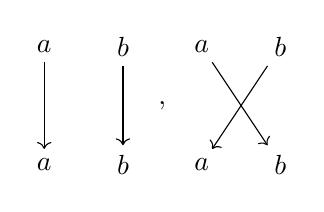
\begin{tikzpicture}[baseline={(current bounding box.center)}]
        % First mapping
        \node (a) at (0,0) {$a$};
        \node (b) at (1,0) {$b$};
        \node (a1) at (0,-1.5) {$a$};
        \node (b1) at (1,-1.5) {$b$};
        \draw[->] (a) -- (a1);
        \draw[->] (b) -- (b1);

        \node (c) at (1.5, -0.75) {$,$};
        % Second mapping
        \node (a) at (2,0) {$a$};
        \node (b) at (3,0) {$b$};
        \node (a1) at (2,-1.5) {$a$};
        \node (b1) at (3,-1.5) {$b$};
        \draw[->] (a) -- (b1);
        \draw[->] (b) -- (a1);
    \end{tikzpicture}
    \right\}
    \]
    $|S_\Omega| = 2.$
\end{eg}
\begin{eg}
    If $\Omega = \{a, b, c\}$, $|S_\Omega| = 6.$
\end{eg}
Order of $S_n$ is $n!$. Let $\sigma \in S_n$, then\\
$\sigma(1)$ has $n$ choices to send $1$ to any $n$ element.\\
$\sigma(2)$ has $(n-1)$ choices.\\
$\sigma(3)$ has $(n-2)$ choices.\\
.\\
.\\
.\\
$\sigma(n)$ has $(1)$ choices.\\
Hence, there is precisely $n(n-1)(n-2)\cdots2\cdot1 = n!$ bijections from $n$ to itself.\\
\begin{definition}
    A \textit{cycle} is a string of integers which represents the element of $S_n$ which cyclically permutes these integers (and fixes all other integers). 
\end{definition}
Let \[\sigma = \begin{pmatrix}
    1 & \rightarrow & 2\\
    2 & \rightarrow & 3\\
    3 & \rightarrow & 1
\end{pmatrix} \in S_3.\]
$\sigma^3 = e$. $\sigma$ is called cycle of length $|\sigma| = 3$ generated by $\sigma$.\\
Again, let $\sigma \in S_5$ and $\sigma$ acts as follows:
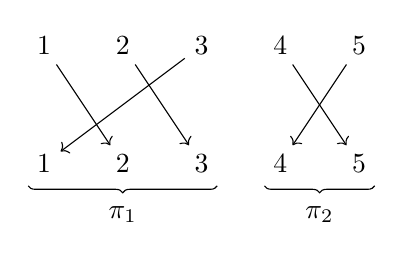
\begin{tikzpicture}[baseline={(current bounding box.center)}]
    % First mapping
    \node (a) at (0,0) {$1$};
    \node (b) at (1,0) {$2$};
    \node (c) at (2,0) {$3$};
    \node (d) at (3,0) {$4$};
    \node (e) at (4,0) {$5$};
    \node (a1) at (0,-1.5) {$1$};
    \node (b1) at (1,-1.5) {$2$};
    \node (c1) at (2,-1.5) {$3$};
    \node (d1) at (3,-1.5) {$4$};
    \node (e1) at (4,-1.5) {$5$};

    % Arrows
    \draw[->] (a) -- (b1);
    \draw[->] (b) -- (c1);
    \draw[->] (c) -- (a1);
    \draw[->] (d) -- (e1);
    \draw[->] (e) -- (d1);

    % Brackets and labels
    \draw[decorate,decoration={brace,mirror,raise=-12pt}] (-0.2,-2.2) -- (2.2,-2.2) node[midway,below=-8pt] {$\pi_1$};
    \draw[decorate,decoration={brace,mirror,raise=-12pt}] (2.8,-2.2) -- (4.2,-2.2) node[midway,below=-8pt] {$\pi_2$};
\end{tikzpicture}\\
$\sigma = \pi_1 \circ \pi_2$, where $\pi_1$ has the cycle structure $(3+1+1)$ and $\pi_2$ has the cycle structure $(2+1+1+1)$.\\
Two cycles are called \textit{disjoint} if they have no elements in common. $\pi_1, \pi_2$ are examples of disjoint cycles. Notice, \textit{two dijoint cycles commutes} as we can see they do not interact with each other.
\begin{theorem}
    Every elements in $S_n$ can be written as composition of disjoint cycles.
\end{theorem}

   \chapter{20 Nov 2024}
   \section{Cycle Notation}
\textbf{Cycle Notation:} The cycle which sends $a_i$ to $a_{i+1}, 1 \le i \le m-1$ and sends $a_m$ to $a_1$ is written as  $(a_1, a_2 ... a_m)$.
\begin{eg}[Cycle Decomposition Algorithm]  
Let $n = 13$ and let $\sigma \in S_{13}$ be defined by
\[
\sigma(1) = 12, \quad \sigma(2) = 13, \quad \sigma(3) = 3, \quad \sigma(4) = 1, \quad \sigma(5) = 11,
\]
\[
\sigma(6) = 9, \quad \sigma(7) = 5, \quad \sigma(8) = 10, \quad \sigma(9) = 6, \quad \sigma(10) = 4,
\]
\[
\sigma(11) = 7, \quad \sigma(12) = 8, \quad \sigma(13) = 2.
\]

\begin{center}
    \def\arraystretch{2}
    \begin{tabular}{|p{0.55\textwidth}|p{0.45\textwidth}|}
    \hline
    \textbf{Method} & \textbf{Example} \\ \hline
    To start a new cycle, pick the smallest element of $\{1, 2, \ldots, n\}$ which has not yet appeared in a previous cycle --- call it $a$ (if you are just starting, $a = 1$); begin the new cycle: $(a$ & $(1$ \\ \hline
    Read off $\sigma(a)$ from the given description of $\sigma$ --- call it $b$. If $b = a$, close the cycle with a right parenthesis (without writing $b$ down); this completes a cycle --- return to step 1. If $b \neq a$, write $b$ next to $a$ in this cycle: $(a\ b$ & $\sigma(1) = 12 = b,  12 \neq 1  \text{ so write: }  (1\ 12$ \\ \hline
    Read off $\sigma(b)$ from the given description of $\sigma$ --- call it $c$. If $c = a$, close the cycle with a right parenthesis to complete the cycle --- return to step 1. If $c \neq a$, write $c$ next to $b$ in this cycle: $(a\ b\ c$. Repeat this step using the number $c$ as the new value for $b$ until the cycle closes. & $\sigma(12) = 8, \ 8 \neq 1 \ \text{ so cycle runs:} \ (1\ 12\ 8$ \\ \hline
    Naturally, this process stops when all the numbers from $\{1, 2, \ldots, n\}$ have appeared in some cycle. & $\sigma = (1 \ 12 \ 8 \ 10 \ 4)(2 \ 13)(3)(5 \ 11 \ 7)(6 \ 9)$\\ \hline
    Final Step: Remove all cycles of length $1$ & $\sigma = (1 \ 12 \ 8 \ 10 \ 4)(2 \ 13)(5 \ 11 \ 7)(6 \ 9)$ \\ \hline
    \end{tabular}
\end{center}
\end{eg}
\begin{eg}[Computing Products in $S_n$]
    While computing products in $S_n$ one reads the permutations from \textit{right to left}. Let's compute $(1 \ 2 \ 3) \circ (1 \ 2)(3 \ 4)$.
    \begin{align*}
        \text{Reading off permutations} & \ \ \ \text{Computing product}\\
        1 \rightarrow 2 \rightarrow 3 & \ \ \ (1 \ 3\\
        3 \rightarrow 4 & \ \ \ (1 \ 3 \ 4\\
        4 \rightarrow 1 & \ \ \ (1 \ 3 \ 4)
    \end{align*}
    Hence, $(1 \ 2 \ 3) \circ (1 \ 2)(3 \ 4) = (1 \ 3 \ 4).$
\end{eg}
\textit{$S_n$ is non-abelian group for all $n \ge 3$.}
\section{Cyclic Permutation, Transposition \& Alternating Group}
\begin{definition}[Cyclic Permutation]
    $\pi \in S_\Omega$ has a cycle of length $r$, and all other cycles are of length $1$, then, $\pi$ is a \textit{cyclic permutation}.
\end{definition}
\begin{definition}[Transposition]
    A cyclic permutation of length $2$ is called a \textit{transposition}.
\end{definition}
\begin{prop}
    Any $r$ cycle can be decomposed into a product of $(r-1)$ transpositions.
\end{prop}
\begin{eg}
    Let $\tau = (1 \ 3 \ 4 \ 6 \ 7 \ 9) \in S_9$\\
    Method 1: $\tau = (1 \ 3 \ 4 \ 6 \ 7 \ 9) = (1 \ 9)(1 \ 7)(1 \ 6)(1 \ 4)(1 \ 3)$\\
    Method 2: $\tau = (1 \ 3 \ 4 \ 6 \ 7 \ 9) = (1 \ 3)(3 \ 4)(4 \ 6)(6 \ 7)(7 \ 9)$\\
    Both products of transpositions method $1$ or method $2$ represent the same permutation $\tau$. Note that the order of the disjoint cycle $\tau$ is $\tau$ but in both expressions of $\tau$ as the product of transpositions, $\tau$ has $5$ (odd numnber of) permutations.  Hence $\tau$ is an \textit{odd permutation}. Similarly, if a permutation is the product of an even number of transpositions, it is called \textit{even permutation}.
\end{eg}
\begin{definition}[Alternating Group]
    Let $A_n$ be the subset of $S_n$ consisting of all even permutations. Since product of two even permutations is even, $A_n$ is a subgroup of $S_n$. $A_n$ is called the \textit{alternating group} of degree $n$.
\end{definition}
   \chapter{2 Dec 2024}
   \section{Normal Subgroup}
\begin{definition}[Normal Subgroup]
    Let $G$ be a group. A subgroup $N$ of $G$ is a normal subgroup if $gN = Ng$, for all $g \in G$. Equivalently, a subgroup $N$ is normal in the group $G$ if $gNg^{-1} = N$, for all $g \in G$. We denote $N\lhd G$.
\end{definition}
\begin{eg}
    $A_3$ is normal in $S_3$. Because, $A_3$ has index 2 in $S_3$, meaning $A_3$ has exactly two cosets: $A_3$ and its complement in $S_3$. Hence, left and right cosets coincide.
\end{eg}
In general, $A_n$ is normal in $S_n$. Furthermore, a subgroup of index 2 is always normal because the left and right cosets coincide.
\begin{eg}[Trivial Examples]
    $\{e\} \in G$ and the group $G$ itself is normal in $G$. 
\end{eg}
\begin{eg}[Center of $G$]
    \hyperref[def:center]{Center} of the group $G$ is a normal subgroup.
\end{eg}
\begin{remark}
    Is every abelian subgroup normal? No.\\
    \textbf{Counter example:} $\{e, s\} \in D_3$ is abelian subgroup. But not normal, since, for instance, $r\{e, s\} \neq \{e, s\}r$.
\end{remark}
\section{Quotient Group}
\begin{theorem}
    Let $N\lhd G$. If $g_1N = g_1'N$ and $g_2N = g_2'N$, then $g_1g_2N = g_1'g_2'N$.
\end{theorem}
\begin{proof}
Let $x \in g_1g_2N$, then $x = g_1g_2n$, for some $n \in N$. Since, $g_2N = g_2'N = Ng_2'$, $g_2n = g_2'n_1 = n_2g_2'$ for some $n_1, n_2 \in N$. So, $x = g_1g_2'n_1 = g_1n_2g_2'$. $g_1n_2 = g_1'n_3$, for some $n_3 \in N$. Hence, $x = g_1'n_3g_2' = g_1'g_2'n'$, for some $n' \in N$. Hence, $x \in g_1'g_2'N$, which implies $g_1g_2N \subseteq g_1'g_2'N$.\\
Using similar argument, $g_1'g_2'N \subseteq g_1g_2N$. Hence, $g_1g_2N = g_1'g_2'N$.
\end{proof}
Cosets of a subgroup $N$ in a group $G$ naturally partition $G$. However, not all subgroups allow these cosets to have a meaningful group structure. When $N$ is a normal subgroup ($gN=Ng$ for all $g \in G$), we can define an operation on cosets that mimics the group operation in $G$. Specifically: $$(gN) \cdot (hN)=(gh)N.$$
This operation is well-defined only if $N$ is normal, ensuring that the choice of representatives $g$ and $h$ does not affect the result as the previous theorem asserts.
\begin{definition}[Coset Multiplication]
    \label{def:quotientop}
    Let $N \lhd G$. Then define a multiplication $\cdot$ on two cosets of $N$ via-
    $$g_1N \cdot g_2N:=g_1g_2N$$
\end{definition}
\begin{theorem}[Quotient Group]
    Under the multiplication operation \hyperref[def:quotientop]{above}, the set of all cosets of the normal subgroup $N$ forms a group, called the \textit{quotient group of $G$ modulo $N$} and denoted as $G/N$.
\end{theorem}
\begin{proof}
    To show that \( G/N \) forms a group under coset multiplication, we verify the group axioms: closure, associativity, identity, and inverses.
    
    \begin{enumerate}
        \item \textbf{Closure:}  
        Let \( g_1N, g_2N \in G/N \). Then their product is defined as:
        \[
        (g_1N)(g_2N) = g_1g_2N.
        \]
        Since \( g_1g_2 \in G \), it follows that \( g_1g_2N \in G/N \). Thus, \( G/N \) is closed under this operation.
    
        \item \textbf{Associativity:}  
        Let \( g_1N, g_2N, g_3N \in G/N \). Then:
        \[
        \big((g_1N)(g_2N)\big)(g_3N) = (g_1g_2N)(g_3N) = (g_1g_2g_3)N.
        \]
        Similarly:
        \[
        (g_1N)\big((g_2N)(g_3N)\big) = (g_1N)(g_2g_3N) = (g_1g_2g_3)N.
        \]
        Therefore, coset multiplication is associative.
    
        \item \textbf{Identity:}  
        The coset \( eN \), where \( e \) is the identity element of \( G \), acts as the identity in \( G/N \). For any \( gN \in G/N \):
        \[
        (eN)(gN) = egN = gN, \quad \text{and} \quad (gN)(eN) = geN = gN.
        \]
        Thus, \( eN \) is the identity element in \( G/N \).
    
        \item \textbf{Inverses:}  
        For any \( gN \in G/N \), the coset \( g^{-1}N \) serves as its inverse. We verify:
        \[
        (gN)(g^{-1}N) = g(g^{-1})N = eN, \quad \text{and} \quad (g^{-1}N)(gN) = g^{-1}gN = eN.
        \]
        Hence, every element in \( G/N \) has an inverse.
    \end{enumerate}
    
    Since \( G/N \) satisfies the group axioms, it forms a group under the given multiplication operation.
    \end{proof}
   \chapter{4 Dec 2024}
   If $G$ is a finite group and $N$ is normal subgroup of $G$, then $$|G/N| = [G:N] = \frac{|G|}{|N|}$$
\begin{eg}
    Let $N = \{e\}$, then $G/N \cong G$.
    Again if $N = G$, then $G/N \cong \{e\}$.\\
    \textbf{Note:} We will learn what $\cong$ means shortly.
\end{eg}
\begin{eg}
 Let $G = (\Z, +)$. Then $n\Z = \{nk: k \in \Z\}$ is normal in $\Z$. Because for all $g \in \Z, g + n\Z + (-g) = n\Z$. Now, let $N = n\Z$. Then distinct cosets of $n\Z$ are:
 \begin{align*}
    \overline{0} &= 0 + n\Z\\
    \overline{1} &= 1 + n\Z\\
    &\vdots\\
    \overline{n-1} &= (n-1) + n\Z
 \end{align*}
 We denote the quotient group as $\Z/n\Z = \{\overline{0}, \overline{1}, \cdots, \overline{n-1}\}$. Notice, from the definition, coset multiplication here is: $(a + n\Z) + (b + n\Z) = a + b + n\Z$ which is exactly how we initially defined the operation on $\Z/n\Z$, i.e., $\overline{a} + \overline{b} = \overline{a + b}$.
\end{eg}
\begin{eg}
    $G = \R$ and $N = 2\pi \Z$. Then, $G/N = \{\theta +2\pi \Z: 0 \le \theta < 2\pi\}$. And multiplication would be like $(\theta_1 + 2\pi\Z) + (\theta_2 + 2\pi\Z) = (\theta_1 + \theta_2 + 2\pi\Z)$.
\end{eg}
\begin{eg}
    We know $A_n$ is a normal subgroup of $S_n$. And since index of $A_n$ in $S_n$ is $2$, $A_n$ has two cosets: $eA_n, (1 \ 2)A_n$. Cayley table for the quotient group modulo $A_n$ is:
    $$
    \begin{tabular}{ |c|c|c| } 
        \hline
        $\cdot$ & $eA_n$ & $(1 \ 2)A_n$  \\
        \hline
        $eA_n$  & $eA_n$  & $(1 \ 2)A_n$  \\
        \hline
        $(1 \ 2)A_n$ & $(1 \ 2)A_n$  & $eA_n$  \\ 
        \hline
    \end{tabular}
    $$
\end{eg}
\section{Group Homomorphism}
Group homomorphism between two groups is aptly called \textit{structure preserving} map as it respect their algebraic structure.
\begin{definition}[Group Homomorphism]
    Given two groups, $(G, *)$ and $(H, \cdot)$, a \textit{group homomorphism} is a map $f: G \rightarrow  H$ such that for all $g_1, g_2 \in G$, $$f(g_1 * g_2) = f(g_1) \cdot f(g_2).$$
\end{definition}
\begin{definition}[Isomorphism]
    A group homomorphism that is bijective is called \textit{isomorphism}.
\end{definition}
When two groups are isomorphic (there's an isomorphism between those groups), they are essentially the same. They differ in that their elements are labeled differently. The isomorphism gives us the key to the labeling, and with it, knowing a given computation in one group, we can carry out the analogous computation in the other. If two groups $G, H$ are isomorphic, we write $G \cong H$.
\begin{prop}
    If $f:G \rightarrow H$ is a homomorphism, then:
    \begin{enumerate}
        \item $f(e_G) = e_H$;
        \item $f(x^{-1}) = f(x)^{-1}$, for all $x \in G$.
    \end{enumerate}
\end{prop}
\begin{propproof}
    To prove $(1)$ we calculate, 
    \begin{align*}
        &f(e_G * e_G) = f(e_G) \cdot f(e_G)\\
        &\implies f(e_G) = f(e_G) \cdot f(e_G)\\
        &\implies f(e_G) \cdot f(e_G)^{-1} = f(e_G) \cdot f(e_G) \cdot f(e_G)^{-1}\\
        &\implies e_H = f(e_G)
    \end{align*}
    To prove $(2)$,
    \begin{align*}
        &f(xx^{-1}) = f(e_G) = e_H\\
        \implies &f(x)f(x^{-1}) = e_H\\
        \implies &f(x^{-1}) = f(x)^{-1}
    \end{align*}
\end{propproof}
\begin{eg}
    $f:G \rightarrow \{e\}$ is homomorphism.
\end{eg}
\begin{explanation}
    For all $g_1, g_2 \in G,$
    \[f(g_1g_2) = e.\]
    Then,
    \[f(g_1) \cdot f(g_2) = e \cdot e = e.\]
\end{explanation}
\begin{eg}
    Let $G = (R, +), H = (R^\times, \times).$\\
    Define $f:G \rightarrow H$ such that $f(x) = e^x$. $f$ is a homomorphism, but not isomorphism.
\end{eg}
\begin{explanation}
    For all $x,y \in \R,$
    \begin{align*}
        f(x + y) &= e^{x+y}\\
        &= e^x \times x^y\\
        &= f(x) \times f(y).
    \end{align*}
    The map is not isomorphism because it is not surjective, e.g., there's no $x\in G$ such that $f(x) = -1 \in H$.
\end{explanation}
   \chapter{9 Dec 2024}
   \section{Kernel and Image of Group Homomorphism}
Let $G$ and $H$ be groups and let $f$ be a group Homomorphism from $G$ to $H$ (Next few lectures will be assuming this statement). Then,
\begin{definition}[Kernel]
    If $e_H$ is the identity element of $H$, then we define \textit{kernel} of $f$ is the preimage of the singleton set $\{e_H\}$. In symbols:
    \[\ker f := \{g \in G: f(g) =e_H\}.\]
\end{definition}
and
\begin{definition}[Image]
    We define \textit{image} of $f$ to be all elements of $H$ which are image of some element of $G$.
    \[\im f := f(G) = \{h \in H: f(g) = h; \text{ for some } g \in G\}\]
\end{definition}
\begin{lemma}
    ker $f$ and Im $f$ are subgroups of $G$ and $H$ respectively.
\end{lemma}
\begin{lemmaproof}
    $f(e_G) = e_H$, hence $e_G \in \ker f$.\\
    Let $x, y \in \ker f$. Then, $f(xy^{-1}) = f(x) f(y^{-1}) = f(x)f(y)^{-1} = e_He_H^{-1} = e_H$.
    According to subgroup criterion, ker $f$ is a subgroup of $G$.\\
    We will prove second part shortly.
\end{lemmaproof}
\begin{lemma}
    ker $f$ is a normal subgroup of $G$.
\end{lemma}
\begin{lemmaproof}
    For all $x \in \ker f$.
    \begin{align*}
        f(g x g^{-1}) &= f(g) f(x) f(g^{-1})\\
                    &= f(g) e_H f(g)^{-1}\\
                    &= f(g) f(g)^{-1}\\
                    &= e_H.
\end{align*}
\end{lemmaproof}
\begin{lemma}
    \label{def:injectivehomo}
    $f$ is injective if and only if ker $f = \{e_G\}$.
\end{lemma}
\begin{lemmaproof}
    ($\implies$)\\
    If $f$ is injective, then, image of every elements of $G$ is unique. Hence, $f(x) = e_H$ if and only if $x = e_G$. Hence, ker $f = \{e_G\}$.\\
    ($\Leftarrow$)\\
    Assume \begin{align*}
        &f(x) = f(y)\\
        \implies & f(x) f(y)^{-1} = e_H\\
        \implies & f(x) f(y^{-1}) = e_H\\
        \implies & f(xy^{-1}) = e_H
    \end{align*}
    Since, ker $f = \{e_G\}$, it must be that $xy^{-1} = e_H$ which implies $x=y$.\\
    Hence, $f$ is injective.
\end{lemmaproof}
\begin{lemma}
    Let $N \lhd G$, then the canonical map $\pi_N: G \rightarrow G/N$ such that $\pi_N(a) = aN$ is a surjective homomorphism with ker $\pi_N = N$.
\end{lemma}
\begin{lemmaproof}
    The map $\pi_N$ is well-defined because for any $a \in G$, the coset $aN$ is uniquely determined. There is no ambiguity in assigning $\pi_N(a) = aN$.\\
    Let $a, b \in G$. Since $N$ is normal in $G$, then $\pi_N(ab) = abN = aN bN = \pi_N(a)\pi_N(b)$. Hence, $\pi_N$ is a homomorphism.\\
    Lastly, identity of $G/N$ is $N$. We know $nN = N$ iff $n\in N$. Hence, ker $f = N$.
\end{lemmaproof}
\begin{corollary}
    A subgroup $N$ is normal if and only if it is the kernel of a group homomorphism.
\end{corollary}
   \chapter{11 Dec 2024}
   \begin{prop}
    If $A \le G$, then $f(A) \le H$. In particular, Im $f = f(G) \le H$.
\end{prop}
\begin{propproof}
    $f(A)$ is non-empty since $e_H \in f(A)$.\\
    Let $x, y \in f(A)$, then $x=f(a_1), y=f(a_2)$, for $a_1, a_2 \in A$.\\
    We know $a_1a_2^{-1} \in A$, therefore, $f(a_1a_2^{-1}) \in f(A).$\\
    Now, $xy^{-1} = f(a_1)f(a_2)^{-1} = f(a_1)f(a_2^{-1}) = f(a_1a_2^{-1}) \in f(A).$\\
    According to subgroup criterion, $f(A) \le H$.
\end{propproof}
\begin{prop}
    Let $f^{-1}(B) = \{x \in G: f(x) \in B\}$. Then, if $B \le H$, then $f^{-1}(B) \le G$. Furthermore, if $B \lhd H$, then $f^{-1}(B) \lhd G$.
\end{prop}
\begin{propproof}
    \textbf{Part 1}\\
    We need to show that \( f^{-1}(B) \) is a subgroup of \( G \).\\
    Firstly, \( f^{-1}(B) \) is nonempty because $e_G \in f^{-1}(B).$\\
    Now, let \( x, y \in f^{-1}(B) \). Then \( f(x), f(y) \in B \). Since \( B \) is a subgroup of \( H \), $f(y)^{-1} \in B$, so:
    $$f(x) f(y)^{-1} = f(x) f(y^{-1}) = f(xy^{-1}) \in B.$$
    Thus, \( xy^{-1} \in f^{-1}(B) \), showing that \( f^{-1}(B) \le G\).\\
    \textbf{Part 2}\\
    We need to show that for all $g \in G$ and $x \in f^{-1}(B)$, $gxg^{-1} \in f^{-1}(B)$. \( x \in f^{-1}(B) \), so \( f(x) \in B \). Let's show $f(gxg^{-1}) \in B$.
    We have:
    \[
    f(gxg^{-1}) = f(g) f(x) f(g^{-1}) = f(g) f(x) f(g)^{-1}.
    \]
    Since \( f(x) \in B \) and \( B \) is normal in \( H \) (i.e., \( B \) is invariant under conjugation), we have:
    \[
    f(g) f(x) f(g)^{-1} = f(gxg^{-1})\in B.
    \]
    Thus, \( f(gxg^{-1}) \in B \), which implies \( gxg^{-1} \in f^{-1}(B) \).\\
    Hence, $f^{-1}(B) \lhd G$.
\end{propproof}
\section{Isomorphism Theorems}
\makebox[0pt][l]{%
\begin{tabular}{@{}m{0.65\textwidth}@{\hspace{1cm}}m{0.3\textwidth}@{}}
    {\small
    \textbf{Emmy Noether (1882–1935)} was one of most influential mathematicians of the 20th century known for her groundbreaking contributions in abstract algebra and theoretical physics. In 1927, she first introduced three isomorphism theorems (sometimes called Noether's isomorphism theorems) of group theory that generalize earlier ideas of abstract algebra. Noether's work exemplified abstraction and generalization. She moved mathematics away from computational techniques and concrete problems toward a more conceptual and unified framework. This approach is now a hallmark of pure mathematics.
    } &
    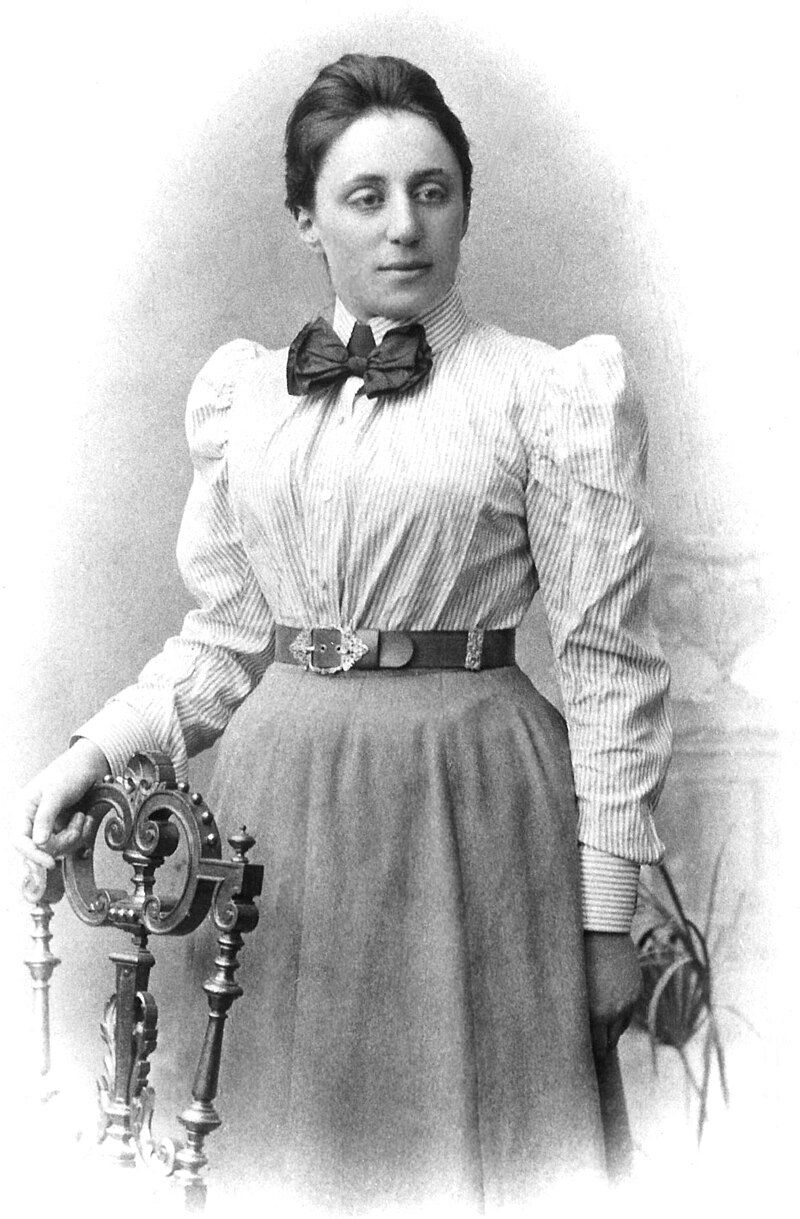
\includegraphics[width=\linewidth]{figures/Noether.jpg} 
\end{tabular}
}
\begin{theorem}[First Isomorphism Theorem]
    Let $f: G \rightarrow H$ be a group homomorphism. Then, there exits an injective homomorphism $f':G/\ker f \rightarrow H$ such that the following diagram commutes:
    \[
    \begin{tikzcd}
        G \arrow[r, "f"] \arrow[d, "\pi_{\ker f}"'] & H \\
        G / \ker f \arrow[ur, "f'"']
    \end{tikzcd}
    \]
    In particular, $G/\ker f \cong f(G)$.
\end{theorem}
\begin{proof}
    Let $N = \ker f$.\\
    $\pi_N: G \rightarrow G/N$.
    \begin{itemize}[label={}]
        \item \textbf{Define $f'$:} Let $f': G/N \rightarrow H$ such that $f'(aN) = f(a).$ The map is well-defined. Let $X \in G/N$. If $X = gN = g'N$, then $f'(X) = f'(gN) = f(g)$ and also $f'(X) = f'(g'N) = f(g')$. Since $gN = g'N$, it follows that $g = g'n$ for some $n \in N$. Using this, $f(g) = f(g'n) = f(g')f(n)$, and because $n \in \ker f$, we know $f(n) = e_H$. Therefore, $f(g) = f(g')$, so the map is well-defined.
        \item $f'$ is a \textbf{homomorphism:}
        \begin{align*}
            f'(aNbN) &= f'(abN)\\
                     &= f(ab)\\
                     &= f(a)f(b)\\
            \implies f'(aNbN) &= f'(aN) f'(bN)
        \end{align*}
        \item $f'$ \textbf{is injective}: By \hyperref[def:injectivehomo]{this} lemma, we know $f'$ is injective if and only if ker $f' = \{e_{G/N}\} = \{N\}.$ $f'(aN) = f(a) = e_H$ if and only if $a \in \ker f = N$.
        $$\ker f' = \{aN: a\in N\} = \{N\} = \{e_{G/N}\} $$
        Hence, $f'$ is injective.
        \item \textbf{The Diagram Commutes:} For all $g \in G, \pi_{\ker f}(g) = g \ker f$ and $f'(g \ker f) = f(g)$. Hence, $f = f' \circ \pi_{\ker f}$
        \item $f'(G/\ker f) = f(G)$. $f'$ is a homomorphism, $f'$ is injective and $f'$ is surjective onto it's image $f(G)$. Hence, $f'$ is bijective map from $G/\ker f$ to $f(G)$. Hence, $f'$ is an isomorphism from $G/\ker f$ to $f(G)$ which means $f'$ is an isomorphism from $G/\ker f$ to $f(G)$.
        Hence, $G/\ker f \cong f(G)$.
    \end{itemize}
\end{proof}
   \chapter{17 Dec 2024}
   \begin{theorem}[Second Isomorphism Theorem]
    Given a group $G$ with a subgroup $H$ and a normal subgroup $N$, $H/(H \cap N) \cong HN / N$.
\end{theorem}
\begin{proof}
    % Let \(x, y \in HN$ then $x = h_1n_1, y= h_2 n_2, \text{ for } h_1, h_2 \in H, n_1, n_2 \in N\). Then, 
    % \begin{align*}
    %     xy^{-1} &= h_1 n_1(h_2n_2)^{-1}\\
    %          &= h_1n_1n_2^{-1}h_2^{-1}
    % \end{align*}
    % Since, $N$ is a normal subgroup and $n_1n_2^{-1} \in N$, $(n_1n_2^{-1})h_2^{-1} = h_2^{-1}n'$ for $n' \in N$. Hence, \[xy^{-1} = h_1n_1n_2^{-1}h_2^{-1} = h_1h_2^{-1}n' \in HN.\]
    % Using subgroup criterion, $HN$ is a subgroup of $G$.
    It is easy to check $HN \leq G$, $N \lhd HN$ and $(H \cap N) \lhd H$. So we directly move on to proving the isomorphic part.\\
    Define $\phi : H \rightarrow HN / N$ such that $\phi(h) = hN$. $\phi$ is homomorphism because for all $x, y \in H$,
        \[
        \phi(xy) = xy N = xN yN = \phi(x)\phi(y).
        \]
    Suppose $xN \in HN$, and $x = hn, h\in H, n \in N$. Hence, $xN = hnN = hN = \phi(h)$. Hence, im $\phi = \phi(H) = HN/N$.\\
    Now, ker $\phi = \{h \in H : \phi(h) = eN = N\}$. Note that $h \in \ker \phi \implies \phi(h) = N \implies hN = N \implies h \in N \implies h \in (H \cap N)$. Again, if $x \in (H \cap N) \implies x \in N \implies \phi(x) = N$. Hence, ker $\phi = H \cap N$.\\
    Using first isomorphism theorem, $H/(H \cap N) \cong HN / N$.
\end{proof}
\begin{theorem}[Third Isomorphism Theorem]
    Given a group $G$ with normal subgroups $N$ and $H$, such that $N \subseteq H, (G/N)/(H/N) \cong G/H$.
\end{theorem}
\section{Automorphism}
\begin{definition}[Automorphism]
    If $f:G \rightarrow G$ is an isomorphism, we call it an \textit{automorphism}.
\end{definition}
\begin{eg}
    $f:G \rightarrow G$ such that $f(g) = g$ is an automorphism.
\end{eg}
\begin{noneg}
    $f:G \rightarrow G$ such that $f(x) = x^{-1}$ is not an isomorphism.
\end{noneg}
\begin{explanation}
    Because $f$ is not a homomorphism in the first place. For $g_1, g_2 \in G$,
        $f(g_1g_2) = (g_1g_2)^{-1} = g_2^{-1}g_1^{-1} = f(g_2) f(g_1)$ is not always equals to $f(g_1)f(g_2)$.
\end{explanation}
\begin{eg}[Conjugation Action]
    $\varphi : G \rightarrow G$ such that $\varphi(x) = gxg^{-1}$ is an automorphism.
\end{eg}
\begin{explanation}
    Firstly, $\varphi$ is a homomorphism.\\
    For all $x,y \in G$,
    \begin{align*}
        \varphi(xy) &= gxyg^{-1}\\
                    &= gxg^{-1}gyg^{-1}\\
                    &= \varphi(x) \varphi(y)
    \end{align*}
    Then, it is easy to show that $\varphi$ is injective and $|G| = |\im \varphi|$ which proves $\varphi$ is surjective too, hence, an automorphism.
\end{explanation}
\begin{noneg}
    Define for $g \in G$, $\lambda_g: G \rightarrow G$ such that $\lambda_g(a) = ga$. $\lambda_g$ is not an automorphism because it is not a homomorphism although it is a bijective map.
\end{noneg}
\begin{lemma}
    $\lambda_g$ in the previous example defines a permutation of $G$. 
\end{lemma}
\begin{lemmaproof}
    To prove injectivity, let,
    $$\lambda_g(a) = \lambda_g(b) \implies ga = gb \implies a = b.$$
    To prove surjectivity, for any $c \in G, c = g g^{-1}c = \lambda_g(g^{-1}c).$\\
    $\lambda_g$ is bijective and every bijective map from a group to itself is a permutation.
\end{lemmaproof}
\begin{theorem}[Cayley's Theorem]
    Every group is isomorphic to a group of permutations.
\end{theorem}
\begin{proof}
    Define for $g \in G$, $\lambda_g: G \rightarrow G$ such that $\lambda_g(a) = ga$ and $\overline{G} = \{\lambda_g: g \in G\}.$ We want to prove, $\overline{G}$ is a group under composition of permutations and $G \cong \overline{G}.$
    To prove $\overline{G}$ is a group,
    \[\lambda_g \circ \lambda_h(a) = \lambda_g[ha] = gha = \lambda_{gh}(a) \textbf{ (Closure)}\]
    Composition of maps is associative \textbf{(Associativity)}.\\
    \textbf{Inverse} and \textbf{identity} are $\lambda_{g^{-1}}$ and $\lambda_e$ respectively for all $g \in G$.\\
    Now, we will define a bijection $\varphi$. Let $\varphi: G \rightarrow \overline{G}$ such that $\varphi(g) = \lambda_g$.\\
    $\varphi$ is a homomorphism because for $g_1, g_2 \in G, \varphi(g_1g_2) = \lambda_{g_1g_2} = \lambda_{g_1} \circ \lambda{g_2} = \varphi(g_1) \varphi(g_2)$.\\
    Now, $\lambda_e$ is the identity element in $\overline{G}$. Let $x \in \ker \varphi, x \in G$. Then, $\varphi(x) = \lambda_x = \lambda_e$. So, $\lambda_x(g) = \lambda_e(g)$ for $g \in G$ which is equivalent to $xg = g \Leftrightarrow x = e$. Hence, $\ker \varphi = \{e\}$, so $\varphi$ is injective.\\
    And since $|G| = |\overline{G}|$, $\varphi$ is also bijective.\\
    Hence, $\varphi$ is an isomorphism, so $G \cong \overline{G}$.
\end{proof}
\section{Conjugacy Classes}
Let $G$ act on itself by conjugation. We write $g \cdot x = g x g^{-1}$. The conjugacy class of $x$ is given by \[\text{Cl} (x) = \{g x g^{-1}: g \in G\}.\]
\begin{eg}
    Consider
    \[S_3 = \{( \ ), (1 \ 2), (1 \ 3), (2 \ 3), (1 \ 2 \ 3), (1 \ 3 \ 2)\}\]
    \[\text{Cl}((1 \ 2)) = \{(1 \ 2), (1 \ 3),(2 \ 3)\}.\]
    \[\text{Cl}((1 \ 2 \ 3)) = \{(1 \ 2 \ 3), (1 \ 3 \ 2)\}.\]
\end{eg}
\begin{theorem}
    Conjugacy classes preserve the cycle structure in $S_n$.
\end{theorem}
\begin{theorem}
    Therefore, conjugacy classes in $S_n$ corresponds to the partitions of $n$.
\end{theorem}
\begin{eg}
    Consider $S_4$. Number of ways to partition $4$, $P(4) = 5$.
    \begin{align*}
        4 &\longleftrightarrow (1 \ 2 \ 3 \ 4)\\
        3 + 1 &\longleftrightarrow (1 \ 2 \ 3) (4)\\
        2 + 2 &\longleftrightarrow (1 \ 2) (3 \ 4)\\
        2 + 1 + 1 &\longleftrightarrow (1 \ 2) (3) (4)\\
        1 + 1 + 1 + 1 &\longleftrightarrow ( \ ) ( \ ) ( \ ) ( \ )
    \end{align*}
\end{eg}
\begin{theorem}
    Conjugacy classes of $G$ partition the group since conjugation defines an equivalence relation.
\end{theorem}
\begin{proof}
    Define the conjugacy relation on \( G \) as follows: For \( g, h \in G \), we say that \( g \sim h \) if there exists some \( x \in G \) such that
    \[
    h = xgx^{-1}.
    \]
    For any \( g \in G \), we can take \( x = e \), the identity element of \( G \). Then,
    \[
    xgx^{-1} = ege = g.
    \]
    Thus, \( g \sim g \), so the relation is \textbf{reflexive}.\\
    Let \( g \sim h \), meaning that there exists an element \( x \in G \) such that \( h = xgx^{-1} \). We want to show that \( h \sim g \), i.e., there exists some element \( y \in G \) such that \( g = yhy^{-1} \).
    We can choose \( y = x^{-1} \). Then,
    \[
    yhy^{-1} = x^{-1}(xgx^{-1})x = g.
    \]
    Thus, \( h \sim g \), so the relation is \textbf{symmetric}.\\
    Let \( g \sim h \) and \( h \sim k \), meaning that there exist elements \( x, y \in G \) such that \( h = xgx^{-1} \) and \( k = yhy^{-1} \). We want to show that \( g \sim k \), i.e., there exists some element \( z \in G \) such that \( k = zgz^{-1} \).
    Substitute \( h = xgx^{-1} \) into the expression for \( k \):
    \[
    k = yhy^{-1} = y(xgx^{-1})y^{-1} = (yx)g(x^{-1}y^{-1}).
    \]
    Let \( z = yx \). Then we have
    \[
    k = zgz^{-1},
    \]
    so \( g \sim k \). Thus, the relation is \textbf{reflexive}.\\
    Therefore, Conjugacy relation is an equivalence relation on \( G \).\\
    The equivalence classes under this relation are called the \textit{conjugacy classes} of \( G \) which partition $G$.
\end{proof}

   \chapter{18 Dec 2024}
   \section{Class Equation}
\begin{definition}
    Stab$(x) = \{g \in G: g \cdot x = x\}$.
\end{definition}
For conjugation action, 
\[
\text{Stab} (x) = \{g\in G: gxg^{-1} = x\} = C_G(x).
\]
\begin{theorem}
    $|\text{Cl}(a)| = [G: \text{Stab}(a)] = [G:C_G(a)] = \frac{|G|}{|C_G(a)|}.$
\end{theorem}
\begin{proof}
    Since \([G : C_G(a)]\) is the number of left cosets of \( C_G(a) \), we want to define a bijective map between elements in \( \text{Cl}(a) \) and the left cosets of \( C_G(a) \).\\
    Let \( H = C_G(a) \).\\
    Since the elements of \( \text{Cl}(a) \) are conjugates of \( a \), we define \( f \) by:
    \[
    f(xa x^{-1}) \mapsto xH
    \]
    We claim that \( f \) is 1-1. Suppose \( f(x) = f(y) \), then \( xH = yH \), and thus \( xh = y \) for some \( h \in H \). But then \( x^{-1}y \in H \), so that \( x^{-1}y \) commutes with \( a \), and therefore:
    \[
    x^{-1}y a = a x^{-1}y.
    \]
    From this, we conclude that:
    \[
    x a x^{-1} = y a y^{-1},
    \]
    which proves that \( f \) is injective.\\
    As for surjectivity, note that for any \( x \in G \), \( x a x^{-1} \) is in \( \text{Cl}(a) \).\\
    However, we also need to show the map is well-defined. That is, we need to show that if \( x a x^{-1} \) and \( y a y^{-1} \) are two descriptions of the same element in \( \text{Cl}(a) \), then \( f(x) = f(y) \). The calculation which shows this is simply the reversal of the steps above. To be precise:
    \[
    x a x^{-1} = y a y^{-1} \quad \Rightarrow \quad a x^{-1} y = x^{-1} y a \quad \Rightarrow \quad x^{-1} y \in H \quad \Rightarrow \quad xH = yH.
    \]
    Thus, the map is well-defined and bijective, so : $|\text{Cl}(a)| = [G : C_G(a)]$.
\end{proof}
\begin{lemma}
    If $x \in Z(G)$, then Cl($x) = \{x\}$.
\end{lemma}
\begin{theorem}[Class Equation]
    Given a finite group $G$ with center $Z(G)$ and representatives $g_1, g_2, ..., g_n$ of the distinct conjugacy classes not contained in $Z(G)$, then 
    \begin{align*}
        |G| &= |Z(G)| + \sum_{i=1}^{n}[G:C_G(g_i)]\\
            &= |Z(G)| + \sum_{i=1}^{n}\frac{|G|}{|C_G(g_i)|}.
    \end{align*} 
\end{theorem}
\begin{proof}
    $\{x\}$ is a conjugacy class of size $1$ if and only if $x \in Z(G)$. Let $Z(G) = \{1, z_1, z_2, ..., z_{k-1}\}$. Since conjugacy classes partition $G$, 
    \[G = (\text{Cl}(z_1) \cup \text{Cl}(z_2) \cup \cdots \cup \text{Cl}(z_k)) \cup (\text{Cl}(g_1) \cup \text{Cl}(g_2) \cup \cdots \cup \text{Cl}(g_n)).\]
    Hence,
    \begin{align*}
        |G| &= |Z(G)| \cdot 1 + \sum_{i=1}^{n}|\text{Cl}(g_i)|\\
            &= |Z(G)| + \sum_{i=1}^{n}[G:C_G(g_i)]\\
            &= |Z(G)| + \sum_{i=1}^{n}\frac{|G|}{|C_G(g_i)|}.
    \end{align*}
\end{proof}
\section{Rings and Fields}
\begin{definition}[Ring]
    A ring $R$ is a set together with two binary operations $+$ and $\times$ (called addition and multiplication respectively) satisfying the following axioms:
    \begin{enumerate}
        \item $(R, +)$ is an abelian group.
        \item $\times$ is associative: $(a \times b) \times c = a \times (b \times c)$ for all $a, b \in R$.
        \item Distributive laws hold: $(a + b) \times c = (a \times c) + (b 
        \times c)$ and $a \times (b + c) = (a \times b) + (a 
        \times c)$ for all $a, b, c \in R$.
    \end{enumerate}
\end{definition}
\begin{remark}[Why we need $(R, +)$ to be abelian group?]
    We need $(R, +)$ to be abelian because otherwise distributive laws will not hold. For instance,
    \[(1+1) \times (a+b) = 1 \times a + 1 \times b + 1 \times a + 1 \times b\]
    But also \[(1+1) \times (a+b) = 1\times a + 1\times a +1 \times b +1 \times b\]
\end{remark}
\begin{definition}[Commutative Ring]
    A ring is said to be \textit{commutative} if multiplication $\times$ is commutative.
\end{definition}
\begin{definition}
    A ring is said to \textit{have an identity} if there is an element $1$ such that 
    \[ 1 \times a = a \times 1 = a \text{, for all } a \in R.\]
\end{definition}
\begin{definition}[Division Ring]
    A ring with identity $1$, where $1 \neq 0$, is called a \textit{division ring}, if every element $a \neq 0 \in R$ has a multiplicative inverse, that is, there exists $b \in G$ such that
    \[a \times b = b \times a = 1.\] 
\end{definition}
\begin{definition}[Field]
    A commutative division ring is called \textit{field}.
\end{definition}
\section{Examples of Ring}
\begin{eg}
    $\Z, \Q, \C, \R$ are all examples of ring and commutative ring. Excluding $\Z$, all of them are division ring, so are fields.
\end{eg}
\begin{eg}[Trivial Ring]
    $\{0\}$ is a \textit{trivial ring}.
\end{eg}
\begin{eg}[Trivial Example]
    For any abelian group R, if we define $a \times b := 0$, then $R$ is a ring.
\end{eg}
   \chapter{19 Dec 2024}
   \section{More Examples of Ring}
\begin{eg}
    $\Z/n\Z$ is an example of a commutative ring because $(\Z/n\Z, +)$ is an abelian group and multiplication modulo $n$ satisfies associativity and commutativity and distributes over addition.
\end{eg}
\begin{eg}
    $\Z/6\Z$ is not a division ring, e.g., $\overline{3}$ doesn't have a multiplicative inverse.
\end{eg}
\begin{eg}[Finite Field]
$\Z/5\Z$ is a division ring. Also it is commutative ring, hence, it is a field.\\
Notice, for all prime numbers $p$, $F_p := \Z/p\Z$ is a field. Number of its elements is finite, hence, it is an example of a finite field.
\end{eg}
\begin{eg}[A ring without multiplicative identity]
    $2\Z$.
\end{eg}
\begin{definition}[Quaternions]
    Let $\mathbb{H}$ to be the set of all quaternions such that 
    \[\mathbb{H} := \{a + bi + cj + dk: a,b,c,d \in R\}.\]
    And define addition $+$ via-
    \[(a_1 + b_1i + c_1j + d_1k)(a_2+b2_i+c_2i + d_2k) := (a_1+a_2) + (b_1 + b_2)i + (c_1+c_2)j + (d_1 + d_2)k.\]
    And multiply using distributive laws subject to the relations:
    \begin{align*}
        &i^2 = j^2 = k^2 = -1\\
        &ij = -ji = k\\
        &jk = -kj = i\\
        &ki = -ik = j
    \end{align*}
\end{definition}
\begin{eg}
The set of all quaternions $\mathbb{H}$ forms a non-commutative division ring.
\end{eg}
\begin{explanation}
\textbf{Quaternions form a ring:}

\begin{itemize}
    \item \textbf{Addition}: The addition of two quaternions is componentwise and is associative and commutative because real numbers are commutative and associative. The additive identity is \( 0 = 0 + 0i + 0j + 0k \), and the additive inverse of \( q = a + bi + cj + dk \) is \( -q = -a - bi - cj - dk \).
    \item \textbf{Multiplication}: The multiplication of quaternions is defined by the distributive law, and is associative.
\end{itemize}
\textbf{Quaternions form a division ring:}
The identity element is \( 1 = 1 + 0i + 0j + 0k \), and every quaternion \( q = a + bi + cj + dk \) has a multiplicative inverse, as shown below. For any non-zero quaternion \( q = a + bi + cj + dk \), the inverse is given by:
\[
q^{-1} = \frac{a - bi - cj - dk}{a^2 + b^2 + c^2 + d^2},
\]
which satisfies \( q q^{-1} = 1 \), as can be verified by multiplying.\\
\textbf{Quaternions form a non-commutative ring:}
By definition, $ij = -ji$, hence, multiplication is not commutative.
\end{explanation}
\begin{eg}[Workout Example]
    $a = 1 + 2j + 3k$ and $b = j + k$.
    \begin{align*}
        a + b &= (1 + 2j + 3k) + (j + k)\\
              &= 1 + (2+1)j + (3+1)k\\
              &= 1 + 3j + 4k.
    \end{align*}
    \begin{align*}
        a \times b &= (1 + 2j + 3k) \times (j + k)\\
                   &= (1 + 2j + 3k)j + (1 + 2j + 3k)k\\
                   &= j + 2j^2 + 3kj + k + 2jk + 3k^2\\
                   &= j + 2(-1) + 3(-i) + k + 2i + 3(-1)\\
                   &= j -2 -3i + k +2i - 3\\
                   &= -5 - i + j + k.
    \end{align*}
\end{eg}
\section{Properties of Ring}
\begin{prop} If $R$ is a ring, then for all $a, b \in R$,
    \begin{enumerate}
        \item $0\cdot a = a \cdot 0 = 0$.
        \item $(-a)b = a(-b) = -(ab)$.
        \item $(-a)(-b) = ab$.
        \item The multiplicative identity is unique.
    \end{enumerate}
\end{prop}
\begin{propproof}
    \begin{enumerate}
        \item \begin{align*}
            (0 + 0) a &= 0\cdot a + 0 \cdot a\\
            \implies 0 \cdot a &= 0\cdot a + 0 \cdot a\\
            \implies 0 &= 0 \cdot a\\
            \implies 0 \cdot a &= 0.
        \end{align*}
        Similarly, $a \cdot 0 = 0$.
        \item \begin{align*}
            (a - a) b &= 0\\
            \implies ab + (-a)b&= 0\\
            \implies (-a)b &= -(ab).
        \end{align*}
        Similarly, $a(-b) = -(ab)$.
        \item Using previous result, $(-a)(-b) = -(a(-b)) = -(-(ab)) = ab.$
        \item Let $1$ and $1'$ be two distinct multiplicative identity. Then for $a \in R$, $a \cdot 1 = a = a \cdot 1'$ which implies $1 = 1'$ (contradiction!). Hence, multiplicative identity has to be unique.
    \end{enumerate}
\end{propproof}
\section{Subring}
\begin{definition}[Subring]
    A subset $S$ of ring $R$ is a \textit{subring} if it is a subgroup of $R$ under addition and if is closed under multiplication.
\end{definition}
\begin{eg}
    $2\Z \subseteq \Z \subseteq \Q \subseteq \R \subseteq \C \subset \mathbb{H}$.
\end{eg}
\section{Characteristic}
\begin{definition}[Characteristic]
    Let $R$ be a ring with identity $1$. If there exists a positive integer $n$ such that $1 + 1 + \cdots + 1 = n1 = 0$, then $n$ is called the characteristic of $R$, and denoted by char($R$). If no such positive integer exists, then $R$ is said to be characteristic zero.
\end{definition}
\begin{eg}
    In $R = \Z/n\Z$, char$(R) = 0$.
\end{eg}
   \chapter{23 Dec 2024}
   \section{Integral Domain}
\begin{definition}[Zero Divisor]
    Let $R$ be a ring. A non-zero element $a \in R$ is called a \textit{zero divisor} if there is a non-zero element $b \in R$ such that either $ab = 0$ or $ba = 0$.
\end{definition}
\begin{eg}
    $\overline{3}$ is a zero divisor in $\Z/6\Z$ since $\overline{3} \cdot \overline{2} = 0$.
\end{eg}
\begin{definition}[Unit]
    Assume $R$ has an identity $1$. An element $u \in R$ is called \textit{a unit in} $R$ if there is some $v \in R$ such that $uv = vu = 1$.
\end{definition}
The set of units in $R$ is denoted by $R^{\times}$.
\begin{eg}
    $\overline{5}$ is a unit in $\Z/6\Z$ since $\overline{5} \cdot \overline{5} = \overline{1}$.
\end{eg}
\begin{definition}[Integral Domain]
    A commutative ring with identity is called an \textit{integral domain} if it has no zero divisor.
\end{definition}
\begin{prop}
    If $R$ is an integral domain, then for all $a,b\in R$,
    \begin{enumerate}
        \item If $ab = 0$ then $a = 0$ or $b = 0$.
        \item If $ab = ac$ then $a = 0$ or $b = c$.
    \end{enumerate}
\end{prop}
\begin{propproof}
    We will prove $2$.
    \begin{align*}
        & ab = ac\\
        &\implies ab - ac = 0\\
        &\implies a(b-c) = 0\\
        &\implies a = 0 \text{ or } b=c.
    \end{align*}
\end{propproof}
\begin{lemma}
    Any finite integral domain is a field.
\end{lemma}
\begin{propproof}
    Let $R$ be a finite integral domain. Hence, $R$ is commutative and has an identity $1$. We just have to prove $R$ is division ring, that, is for every $a \in R$ there is a $b \in R$ such that $ab = 1$.\\
    For $a \neq 0 \in R$ define $\varphi_a:R \rightarrow R$ such that $\varphi_a(x) = ax$.
    Since $a \neq 0$, $\varphi_a$ is injective. Since $R$ is finite, $|\varphi_a(R)| = |R|$. Hence, $\varphi_a$ is also surjective, so, the map is bijective.\\
    Therefore, for all $a \neq 0$, there is $b$, such that $\varphi_a(b) = 1 \implies ab = 1$.\\
    Hence, $R$ is a field. 
\end{propproof}
\newpage
\section{Ring Homomorphisms}
\begin{definition}[Ring Homomorphism]
    A \textit{ring homomorphism} $\varphi: R \rightarrow S$ is a map satisfying the following:
    \begin{enumerate}
        \item $\varphi(a + b)  = \varphi(a)+ \varphi(b)$ for all $a, b \in R$,
        \item $\varphi(a b)  = \varphi(a)\varphi(b)$ for all $a, b \in R$.
    \end{enumerate}
\end{definition}
\begin{definition}[Isomorphism]
    A bijective ring homomorphism is called an \textit{isomorphism}.
\end{definition}
\begin{eg}[Trivial Homomorphism]
    $\varphi: R \rightarrow S$ such that $\varphi(r) = 0$.
\end{eg}
\begin{eg}[Identity Homomorphism]
    $\varphi: R \rightarrow R$ such that $\varphi(r) = r$.
\end{eg}
\begin{eg}
    $\varphi: \Z \rightarrow \Z/n\Z$ such that $\varphi(x) = x \mod n$ is homomorphism.
\end{eg}
\begin{explanation}
    For all $a, b \in \Z$, 
    \begin{align*}
        \varphi(a + b)  &=(a+b) \text{ mod } n\\
                        &= a \text{ mod } n + b \text{ mod } n\\
                        &= \varphi(a) + \varphi(b).
    \end{align*}
    \begin{align*}
        \varphi(a b)  &= ab \text{ mod } n\\
                      &= (a \text{ mod } n) (b \text{ mod } n)\\
                      &= \varphi(a) \cdot \varphi(b).
    \end{align*}
\end{explanation}
\begin{definition}[Polynomial Ring]
    % Let $R$ be a ring. Define $R[x]$ to be the set of all polynomials in $x$ with coefficients in $R$. In symbols,
    % \[R[x] = \{a_nx^n + a_{n-1}x^{n-1} + ... + _1x + a_0 : a_n, a_{n-1}, ..., a_1, a_0 \in R\}.\]
    % $R[x]$ is a ring called \textit{polynomial ring}.
    Let $R$ be a ring, $x$ be an indeterminate and define $R[x]$ be the set of all formal sums
    \begin{align*}
        R[x] := a_nx^n + a_{n-1}x^{n-1} + \cdots + a_1x + a_0 = \sum a_ix^i.
    \end{align*}
    Given two polynomials $f = \sum a_ix^i$ and $g = \sum b_ix^i$ in $R[x]$, the sum of $f$ and $g$ is defined as
        \[f + g = \sum (a_i + b_i)x^i,\]
    (where we have implicitly assumed that $m \leq n$ and we set $b_i = 0$ for $i > m$).
    And the product of $f$ and $g$ as
    \[fg = \sum_{i}^{}(\sum_{j}^{}a_jb_{i-j})x^i.\]
    With this rule of addition and multiplication, $R[x]$ becomes a ring, called \textit{polynomial ring}. 
\end{definition}
In the definition above, each $a_i \in R$ is called the coefficients of the polynomial; $a_i$ is the coefficient of $x^i$ and the zero element given as the polynomial with zero coefficients.
\begin{eg}
    $\varphi: \Q[x] \rightarrow \Q$ such that $\varphi(P(x)) = P(0)$ is a ring homomorphism.
\end{eg}
\begin{explanation}
    \begin{align*}
        &\varphi[P_1(x) + P_2(x)]\\
        &= P_1(0) + P_2(0)\\
        &= \varphi[P_1(x)] + \varphi[P_2(x)].
    \end{align*}
     \begin{align*}
        &\varphi[P_1 P_2]\\
        &= P_1P_2(0)\\
        &= P_1(0) P_2(0)\\
        &= \varphi[P_1(x)]  \varphi[P_2(x)].
    \end{align*}
\end{explanation}
\section{Kernel and Image of Ring Homomorphism}
\begin{definition}[Kernel of Ring]
    For rings, the \textit{kernel} is the set of all elements in $R$ that get mapped to $0 \in S$. In symbols,
    \[\ker \varphi = \{r \in R: \varphi(r) = 0\}.\]
\end{definition}
\begin{prop}
    \label{def:kernelisideal}
    Let $R$ and $S$ be rings and $\varphi: R \rightarrow S$ a ring homomorphism. Then,
    \begin{enumerate}
        \item The image of $\varphi$ is a subring of $S$.
        \item ker $\varphi$ is a subring of $R$. Furthermore, ker $\varphi$ is closed under multiplication by every element of $R$.
    \end{enumerate}
\end{prop}
\begin{propproof}
    \begin{enumerate}
        \item Let $a, b \in \im \varphi$, then there is $r_1, r_2 \in R$ such that $a = \varphi(r_1)$ and $b = \varphi(r_2)$. Since $\varphi$ is a homomorphism,
        \[a - b = \varphi(r_1) - \varphi(r_2) = \varphi(r_1 - r_2) \in S.\]
        Hence, im $\varphi$ is closed under subtraction.\\
        Again since $\varphi$ is a homomorphism,
        \[ab = \varphi(r_1)  \varphi(r_2) = \varphi(r_1  r_2) \in S.\]
        Therefore, im $\varphi$ is closed under multiplication.\\
        Hence, im $\varphi$ is a subring of $S$.
        \item Let $a, b \in \ker \varphi$, then $\varphi(a) = 0$ and $\varphi(b) = 0$. Since $\varphi$ is a homomorphism,
        \[\varphi(a - b) = \varphi(a) - \varphi(b) = 0 - 0 = 0.\]
        Hence, $(a-b) \in \ker \varphi$, so ker $\varphi$ is closed under subtraction.\\
        Again since $\varphi$ is homomorphism,
        \[\varphi(ab) = \varphi(a)\varphi(b) = 0 \cdot 0 = 0.\]
        Therefore, $ab \in \ker \varphi$, so ker $\varphi$ is closed under multiplication.\\
        Hence, ker $\varphi$ is a subring of $R$.\\
        Now, for the last part, let \( a \in \ker(\varphi) \) and \( r \in R \). Then \( \varphi(a) = 0 \). Since \( \varphi \) is a ring homomorphism, we have:
        \[
        \varphi(ra) = \varphi(r) \cdot \varphi(a) = \varphi(r) \cdot 0= 0,
        \]
        and
        \[
        \varphi(ar) = \varphi(a) \cdot \varphi(r) = 0 \cdot \varphi(r) = 0.
        \]
        Thus, \( ra, ar \in \ker(\varphi) \). Hence, \( \ker(\varphi) \) is closed under multiplication by elements of \( R \).
    \end{enumerate}
\end{propproof}
   \chapter{28 Dec 2024}
   \section{Ideals}
Let $R$ be a ring, let $I$ be a subset of $R$ and let $r \in R$. We have two subsets 
\[rI = \{ra: a \in I\}\]
and
\[Ir = \{ar: a \in I\}.\]
\begin{definition}[Left Ideal]
    A subset $I$ of $R$ is a left ideal of $R$ if $I$ is a subring of $R$ and $I$ is closed under left multiplication by elements of $R$, that is, $rI \subseteq I$ for all $r \in R$.
\end{definition}
Similarly we can define,
\begin{definition}[Right Ideal]
    A subset $I$ of $R$ is a right ideal of $R$ if $I$ is a subring of $R$ and $I$ is closed under right multiplication by elements of $R$, that is, $Ir \subseteq I$ for all $r \in R$.
\end{definition}
We say we have a \textit{two-sided ideal} or simply an \textit{ideal} when $I$ is both a left and right ideal. A left idea is not necessarily a right ideal. But in commutative rings, a left ideal is also a right ideal.
\begin{lemma}[Ideal Criterion(?)]
    A subset $I$ of ring $R$ is an ideal if-
    \begin{itemize}
        \item $I$ is non-empty and closed under subtraction.
        \item $I$ is closed under multiplication by any element of $R$.
    \end{itemize}
\end{lemma}
\section{Examples of Ideal}
\begin{eg}
    The kernel of any ring homomorphism is an ideal.
\end{eg}
\begin{explanation}
    Was done in this \hyperref[def:kernelisideal]{proposition}.
\end{explanation}
\begin{eg}
    $n\Z$ is an ideal of $\Z$.
\end{eg}
\begin{explanation}
    $n\Z$ is a subring of $\Z$, which can be easily checked. For any element $x \in n\Z$ and $y \in \Z$, we have \[yx = y \cdot (kn) = yk \cdot n\]
    for some $k \in \Z$. So $yx \in n\Z$, and $n\Z$ is a left ideal. $\Z$ is commutative, so $n\Z$ is also a right ideal.
\end{explanation}
\begin{eg}
    Let $R = \Z[x]$ be the ring of polynomials in $x$ with integer coefficients and $I$ be the set of polynomials whose terms are of degree at least $2$ (i.e., having no terms of degree $0$ and $1$) together with zero polynomial. Then $I$ is an ideal of $R$.
\end{eg}
\begin{explanation}
If \( f, g \in I \), then \( f + g \in I \) since adding polynomials with no terms of degree \( 0 \) or \( 1 \) results in another polynomial with the same property.\\
Then, if \( f \in I \) and \( r \in R \), then \( r \cdot f \in I \) because multiplying any polynomial \( f \) by \( r \) does not introduce terms of degree \( 0 \) or \( 1 \) into \( r \cdot f \).\\
Thus, \( I \) is closed under addition and closed under multiplication by any element of $R$. As \( 0 \in I \), it is non-empty. Therefore, \( I \) is an ideal of \( R \).
\end{explanation}
\begin{eg}
    Let $M_{n \times n}(R)$ be the matrix ring over some ring $R$. If $J$ is an ideal of $R$, $M_{n\times n}(J)$ is an ideal of $M_{n \times n}(R)$.
\end{eg}
\begin{explanation}
    \textbf{Non-empty:} Since \( J \) is an ideal of \( R \), it contains the zero element, i.e., \( 0 \in J \). Therefore, the zero matrix belongs to \( M_{n \times n}(J) \). Hence, \( M_{n \times n}(J) \) is non-empty.\\
Let \( A = (a_{ij}) \) and \( B = (b_{ij}) \) be matrices in \( M_{n \times n}(J) \), where each entry \( a_{ij} \in J \) and \( b_{ij} \in J \).\\
\textbf{Closure under subtraction:} Consider the matrix \( A - B \):
\[
A - B = (a_{ij} - b_{ij}).
\]
Since \( J \) is an ideal of \( R \), it is closed under subtraction, so \( a_{ij} - b_{ij} \in J \) for all \( i, j \). Therefore, \( A - B \in M_{n \times n}(J) \).\\
\textbf{Closure under multiplication by any matrix in \( M_{n \times n}(R) \)}
We need to show that both \( AB \in M_{n \times n}(J) \) and \( BA \in M_{n \times n}(J) \).\\
\textbf{Left multiplication by \( B \):}\\
Let \( C = AB \), where the entry \( c_{ij} \) in the matrix \( C \) is given by
\[
c_{ij} = \sum_{k=1}^{n} a_{ik} b_{kj}.
\]
Since \( a_{ik} \in J \) (because \( A \in M_{n \times n}(J) \)) and \( J \) is an ideal of \( R \), and \( b_{kj} \in R \), the product \( a_{ik} b_{kj} \in J \) because \( J \) is closed under multiplication by any element of \( R \). Hence, each entry \( c_{ij} \in J \), implying \( C = AB \in M_{n \times n}(J) \).\\
\textbf{Right multiplication by \( A \):} Similarly, \( BA \in M_{n \times n}(J) \).\\
Since \( M_{n \times n}(J) \) is non-empty, closed under subtraction, and closed under multiplication by any element of \( M_{n \times n}(R) \), it follows that \( M_{n \times n}(J) \) is an ideal of \( M_{n \times n}(R) \).
\end{explanation}
\begin{eg}[All ideals are not two-sided]
    Consider the ring $M_{2\times 2}(R)$, where $R$ is an commutative ring with identity. Let $L_1$ be the set of all matrices in $M_{2 \times 2}(R)$ with only entries in the first column, i.e., 
    \[
    L_1 = \left\{\begin{pmatrix}
    a & 0\\
    b & 0
    \end{pmatrix}: a, b \in R\right\}.
    \]
    Then, $L_1$ is a left ideal, but not right ideal.\\
    We can similarly define $R_1$ which is a right ideal but not a left ideal. We can also define $L_2, R_2$. In general, we can define $L_1, L_2, \cdots, L_n, R_1, R_2, \cdots, R_n$ for $n \times n$ matrices.
\end{eg}
\begin{eg}[Sum of Ideals]
    If $I$ and $J$ are two ideals of $R$, we can take the set $I + J$ defined by
    \[
    I + J = \{a + b: a \in I, b \in J\},
    \]
    which also happens to be an ideal of $R$. This is called the \textit{sum of two} ideals $I$ and $J$.
\end{eg}
\begin{eg}[Product of Two Ideals]
    The \textit{product of two ideals} \(I\) and \(J\) in a ring \(R\), denoted as \(IJ\), is defined as the ideal of $R$ generated by all finite sums of products of elements from \(I\) and \(J\). That is,

    \[
    IJ = \left\langle \sum_{k=1}^n a_k b_k \mid a_k \in I, b_k \in J, n \in \mathbb{N} \right\rangle.
    \]
\end{eg}
\begin{eg}[n-fold Ideal]
    For an ideal \(I\) in a ring \(R\), the \(n\)-fold ideal \(I^n\) is the ideal of $R$ generated by all finite sums of products of \(n\) elements, where each element is taken from \(I\). That is,
    \[
    I^n = \left\langle \sum_{k=1}^m a_1 a_2 \cdots a_n \mid a_1, a_2, \dots, a_n \in I, m \in \mathbb{N} \right\rangle.
    \]
\end{eg}
\section{Quotient Rings}
Just like we defined quotient groups where we mod out by a normal subgroup, for rings we can define quotient rings by \textit{mod}-ing out by an appropriate ideal.
\begin{definition}[Quotient Ring]
    Let $R$ be a ring and let $I$ be an ideal of $R$. Then the (additive) quotient group $R/I$ is a ring under the binary operations:
    \[(r + I) + (r + I) := (r + s) + I\]
    \[(r + I) (s + I) := rs + I,\]
    where $r, s \in R$. $R/I$ is called quotient ring of $R$ modulo $I$.
\end{definition}
\begin{eg}
    Let $R = \Z$ and $I = n\Z$. Then we have $R/I = \Z/n\Z$, the quotient ring of $\Z$ modulo $n\Z$.\\
    We saw earlier that $\Z/n\Z$ is a ring, in particular, is a field when $n$ is prime. 
\end{eg}
\begin{eg}
    Let $R = \Z[x]$ and $I$ be the collection of polynomials whose terms are of degree at least $2$ with the zero polynomial. Two polynomial $p(x), q(x)$ are in the same coset of $I$ if and only if they differ by a polynomial whose terms are of degree at least $2$, i.e., $p(x)$ and $q(x)$ have the same constant and first degree term. Hence, $R/I = \{a + bx: a, b \in R\}$. Furthermore, we add and multiply in this quotient ring as usual and taking $x^2 = 0$ in this ring.\\
    It is interesting to note that $R/I$ has zero divisors though $R$ does not.
\end{eg}
\section{Canonical Projection Map}
If $I$ is any ideal, then $R/I$ is a ring and the canonical map 
\[\pi : r \rightarrow r + I,\]
is a ring homomorphism with kernel $I$.\\
We already know $\pi$ is a group homomorphism, it remains to check that $\pi$ is also ring homomorphism. This is immediate from the definition of multiplication in $R/I$:
\[\pi(rs) = rs + I = (r + I)(s + I) = \pi(r)\pi(s).\]
Hence,
\begin{theorem}
    We can realize every ideal as the kernel of some ring homomorphism.
\end{theorem}
\section{Isomorphism Theorems for Rings}
\begin{theorem}[First Isomorphism Theorem]
    If $\phi: R \rightarrow S$ is a homomorphism of rings, then $R /ker \ \phi$ is isomorphic as a ring to $\phi(R)$.
\end{theorem}
\begin{proof}
    The proof goes same as first Isomorphism theorem proof that we did previously. Here we just have to consider extra ring multiplication operation. If $I = \ker \ \phi$, then the correspondence $r + I \rightarrow \phi(r)$ is a bijection between the rings $R/I$ and $\phi(R)$ which respects addition, in this case, also multiplication, hence is a ring isomorphism. Therefore, $R /ker \ \phi \cong \phi(R)$.
\end{proof}
\begin{eg}
    Let $R = \Z[x]$ and consider the homomorphism $\phi : \Z[x] \rightarrow \Z/2\Z$ such that \[\phi(p(x)) = p(0) \mod \ 2.\] Then $R/ \ker \ \phi \cong \Z/2\Z$.
\end{eg}
\begin{explanation}
    Firstly, $\ker \ \phi = \{p(x) \in \Z[x]: p(0) \in 2\Z\}$ is mapped to $\overline{0} \in \Z/2\Z$. And the set of all polynomials whose constant term is odd mapped to $\overline{1}$. Hence, the homomorphism is surjective. According to the first isomorphism theorem,
    \[R /ker \ \phi \cong \Z/2\Z\]
\end{explanation}
\begin{theorem}[Second Isomorphism Theorem]
    Let $A$ be a subring and let $B$ be an ideal of $R$. Then $A + B = \{a + b : a \in A, b \in B\}$ is a subring of $R$, $A \cap B$ is an ideal of $A$ and $(A + B)/B \cong A/(A \cap B)$.
\end{theorem}
\begin{theorem}[Third Isomorphism Theorem]
    Let $I$ and $J$ be ideals of $R$ with $I \subseteq J$. Then $J/I$ is an ideal of $R/I$ and $(R/I)/(J/I) \cong R/J$. 
\end{theorem}
One can prove both theorems using similar arguments (that were used to prove isomorphism theorems for groups).
   \chapter{30 Dec 2024}
   \section{Ideals Generated By A Subset}
\begin{definition}[Ideal Genereated By A Subset]
Let $A$ be a subset of a ring $R$ with identity $1 \neq 0$. Let $S = \{I_k\}$ be the collection of all left ideals of $R$ that contain $A$ (note that the set is nonempty since $A \subseteq R$ and $R$ is an ideal in itself). The intersection
\[
\bigcap_{I_k \in S} I_k,
\]
is called the \textit{left ideal generated by} $A$, and is denoted by $(A)_L$.
Alternatively, we can constructively form the set of elements that constitutes this ideal: 
\[(A)_L = \left\{\sum_{k=1}^{m}r_ka_k: r_k \in R, a_k\in A, m \in \N\right\}.\]
The definition is symmetrical for \textit{right ideal generated by a subset}.
\end{definition}
\begin{definition}[Finitely Generated Ideal]
    An ideal in a commutative ring is said to be \textit{finitely generated} if there exits $x_1, x_2, ..., x_n$ such that 
    \[I = Rx_1 + Rx_2 + \cdots + Rx_m, m \in \N.\]
    Or for all $i \in I$,
    \[i = r_1 x_1 + r_2 x_2 + \cdots + r_nx_n.\]
\end{definition}
\begin{eg}
    $R = \Z, I = 2\Z + 3\Z = (2,3) = \{2k + 3l: k,l \in \Z\}$. Hence, $2\Z + 3\Z$ is a finitely generated ideal in $\Z$.
\end{eg}
\begin{definition}[Principle Ideal]
    \textit{Principle ideal} is an ideal generated by a single element $a$. Symbolically,
    \[(a) = \{ra: r \in R\}\]
\end{definition}
\begin{eg}
    $R = \Z, I = 3\Z = (3) = \{k \cdot 3 : k \in \Z\}$. Hence, $3\Z$ is a principle ideal in $\Z$.
\end{eg}
\begin{prop}
    Let $I$ be an ideal of $R$ with identity. Then,
    \begin{enumerate}
        \item $I = R$ if and only if $I$ contains the unit element.
        \item $I = R$ if and only if $I$ contains a unit.
        \item Assume $R$ is commutative, then $R$ is a field if and only if its only ideals are $(0)$ and $(1)=R$ itself.
    \end{enumerate}
\end{prop}
\begin{propproof}
    \begin{enumerate}
        \item If $I = R$, then its obvious. Now let $I$ contains $1$, then $r \cdot 1 = r \in I$, for all $r \in R$. Therefore, $R \subseteq I$. But $I \subseteq R$ by definition. Hence, $I = R$.
        \item If $I = R$, then its obvious. Let $a$ be a unit in $R$. Then, there exits $b \in R$ such that $ba = 1$. But since $I$ is an ideal $ba = 1 \in I$. From the previous result, $I = R$.
        \item Let $R$ be a field and $I$ be a nonzero ideal of $R$ and $x \in I$. Then $x x^{-1} = 1 \in I$. Since $1 \in I$, $I = R$. Hence, only ideals of $R$ are $(0)$ and $R$ itself. Conversely, if $(0)$ and $R$ are the only ideals of $R$, let $u$ be any nonzero element of $R$. By hypothesis $(u) = R$ and so $1 \in (u)$. Thus there is some $v \in R$ such that $1 = vu$, which means $u$ is an unit. It is true for all $u \in R$. Hence, $R$ is a commutative division ring, i.e., field. 
    \end{enumerate}
\end{propproof}

   \chapter{4 Jan 2025}
   \section{Maximal Ideals}
\begin{definition}[Maximal Ideal]
    An ideal $M$ in an arbitrary ring $R$ is a \textit{maximal ideal} if $M \neq R$ and the only ideals that contain $M$ are $M$ and $R$.
\end{definition}
In other words, $M \neq R$ is a maximal ideal if there is no other proper ideal of $R$ that contains $M$. $M \subset K \subset R \implies$ either $K = M$ or $K = R$.
\begin{noneg}
    $6\Z$ is not a maximal ideal of $\Z$ because $6\Z \subset 3\Z$.
\end{noneg}
\begin{lemma}
    If $p$ is a prime, then $p\Z$ is a maximal ideal.
\end{lemma}
\begin{lemmaproof}
    Let $p\Z \subset q\Z \subset \Z$. For the inclusion to be true, $q$ must divide $p$. Since $p$ is a prime, either $q=1 \implies q\Z = \Z$ or $q = p \implies q\Z = p\Z$. Which means $p\Z$ is a maximal ideal.
\end{lemmaproof}
\begin{eg}
    $(2,x)$ in $\Z[x]$ is a maximal ideal.
\end{eg}
\begin{explanation}
    $\Z/2\Z$ is a maximal ideal, $(2,x) = \{2p(x) + q(x): p(x), q(x) \in \Z[x]\}$ and $\Z[x]/(2,x) \cong \Z/2\Z$. Hence, $(2,x)$ is a maximal ideal in $\Z$.
\end{explanation}
\begin{noneg}
    $(x) \subset \Z[x]$ is not a maximal ideal since $(x) \subset (2,x) \subset \Z$.
\end{noneg}
\begin{theorem}[Correspondence Theorem]
    Let $R, R'$ be rings and $\varphi$ be a homomorphism from $R$ to $R'$ with kernel $u$. Then there is a one-one correspondence between the set of ideals in $R$ which contain $u$ and the set of ideals in $R'$. 
\end{theorem}
\begin{prop}
    Assume $R$ is commutative. Then $M$ is maximal ideal if and only if $R/M$ is a field.
\end{prop}
\begin{propproof}
    Consider canonical map $\varphi: R \rightarrow R/M$. Then $\varphi$ has kernel $M$.\\
    Assume $M$ is a maximal ideal. Then only two ideals contain $M$: $M$ and $R$. Let $I$ be an ideal in $R/M$. By correspondence theorem, there is an ideal $K \subseteq R$ containing $M$. However, since $M$ is a maximal ideal, either $K = M$ or $K = R$. Therefore, there are only two ideals in $R/M$. They are $(0)$ and $(R/M)$ itself. Hence, $R/M$ is a field.\\
    Conversely, let $R/M$ is a field. Then for all ideal $I$ in $R/M$, there exists a corresponding ideal $K$ in $R$ that contain $M$. But either $I = R/M$ or $I = (0)$. Which means $R$ has two ideals containing $M$, which are $M$ and $R$. Hence, $M$ is a maximal ideal.
\end{propproof}
\section{Prime Ideals}
\begin{definition}[Prime Ideal]
    Assume $R$ is commutative. An ideal $P \subset R$ is called \textit{prime ideal} if $P \neq R$ and whenever $ab \in P$ for $a,b \in R$, then either $a \in P$ or $b \in P$ or both.
\end{definition}
\begin{noneg}
    $6\Z$ is not a prime ideal of $\Z$ because $3 \times 2 = 6 \in 6\Z$ but $2,3 \not \in 6\Z$.
\end{noneg}
\begin{lemma}
    $p\Z$ is a prime ideal in $\Z$.
\end{lemma}
\begin{explanation}
    Let $ab \in p\Z$. Then $ab = pk$ for some $k \in \Z$. By prime factorization, either $p \vert  a$ or $p \vert  b$ or both, which implies either $a \in p\Z$ or $b \in p\Z$ or both.
\end{explanation}
\begin{lemma}
    Every maximal ideal is a prime ideal.
\end{lemma}
The converse of the above lemma does not hold.
\begin{prop}
    Assume $R$ is commutative. An ideal $P \in R$ is a prime ideal if and only if $R/P$ is an integral domain.
\end{prop}
\begin{propproof}
    Assume $P$ is a prime ideal. Let $\overline{a}, \overline{b} \in R/P$ and $\overline{a} \cdot \overline{b} = 0$ which implies $\overline{ab} = 0 \implies ab \in P$.
    Since $P$ is prime, either $a \in P \implies \overline{a}=0$ or $b \in P \implies \overline{b}$ or both. Therefore, according to the definition, $R/P$ is an integral domain.\\\\
    Conversely, assume that $R/P$ is an integral domain. Let $ab \in P$. Then $0 + P = ab + P = (a+P)(b+P)$ which implies that $a+P = 0 +P$ or $b+P = 0 +P$, since $R/P$ is an integral domain. Thus, $a \in P$ or $b \in P$ and so $P$ is a prime ideal. 
\end{propproof}
\section{Fields of Fractions of An Integral Domain}
\begin{definition}[Field of Fractions of an Integral Domain]  
Let \( R \) be an integral domain. Define \( N \subseteq R \times R \) as the set of pairs \( (a, b) \) where \( b \neq 0 \). An equivalence relation \(\sim\) on \( N \) is defined by  
\[
(a, b) \sim (p, q) \iff aq = bp.
\] 
The \textit{field of fractions} of \( R \) is the set of equivalence classes under this relation.\\
We denote the equivalence class of \( (a, b) \) by \([a, b]\). This set forms a field with the following operations:  
\[
[a, b] + [c, d] := [ad + bc, bd].
\]  
\[
[a, b] \cdot [c, d] := [ac, bd].
\] 
\end{definition}
The proof that field of fractions indeed forms a field is simple, but tedious to check. However, it is worth mentioning that the additive and multiplicative identities of such field are given by \([0, 1]\) and \([1, 1]\), respectively.

   \chapter{4 Jan 2025}
   \section{Examples of Field of Fractions}
\begin{eg}
    $\Q$ is the field of fractions of $\Z$.
\end{eg}
\begin{definition}[Gaussian Integers]
    Consider $\Z[i] = \{a + bi: a, b \in \Z\}$ known as \textit{Gaussian integers}. Define
    \[(a+bi) + (c + di) := (a+c)+(b+d)i,\]
    \[(a+bi) \cdot (c + di) := (ac-bd)+(ad + bc)i.\]
    Then, $\Z[i]$ is an integral domain under these operations.
\end{definition}
\begin{eg}
    $\Q[i]$ is the field of fractions of $\Z[i]$.
\end{eg}
\begin{explanation}
    To prove that \(\mathbb{Q}[i]\) is the field of fractions of \(\mathbb{Z}[i]\), we verify the following:
\begin{enumerate}
    \item Every element of \(\mathbb{Q}[i]\) can be expressed as a fraction of elements in \(\mathbb{Z}[i]\).
    \item If an element can be expressed as a fraction of elements in \(\mathbb{Z}[i]\), it belongs to \(\mathbb{Q}[i]\).
\end{enumerate}
\textbf{1.} By definition, \(\mathbb{Q}[i] = \{a + bi \mid a, b \in \mathbb{Q}\}\). 
    Let \(a, b \in \mathbb{Q}\). Since \(\mathbb{Q}\) is the field of fractions of \(\mathbb{Z}\), we can write \(a = \frac{m}{n}\) and \(b = \frac{p}{q}\), where \(m, n, p, q \in \mathbb{Z}\) and \(n, q \neq 0\).\\
    Then, 
    \[
    a + bi = \frac{m}{n} + \frac{p}{q}i = \frac{mq + np i}{nq},
    \]
    where \(mq + np i \in \mathbb{Z}[i]\) and \(nq \in \mathbb{Z} \setminus \{0\}\).\\
    Hence, \(a + bi \in \mathbb{Q}[i]\) is expressible as \(\frac{\alpha}{\beta}\), where \(\alpha, \beta \in \mathbb{Z}[i]\) and \(\beta \neq 0\).\\\\
\textbf{2.}
    Let \(\frac{\alpha}{\beta}\) be a fraction where \(\alpha, \beta \in \mathbb{Z}[i]\) and \(\beta \neq 0\).\\
    Write \(\alpha = a + bi\) and \(\beta = c + di\), where \(a, b, c, d \in \mathbb{Z}\).\\
    The inverse of \(\beta\) in \(\mathbb{Q}[i]\) is given by:
    \[
    \beta^{-1} = \frac{\overline{\beta}}{\beta \overline{\beta}} = \frac{c - di}{c^2 + d^2},
    \]
    where \(\overline{\beta} = c - di\) is the complex conjugate of \(\beta\).\\
    Since \(c^2 + d^2 \neq 0\), \(\beta^{-1} \in \mathbb{Q}[i]\).\\
    Therefore, 
    \[
    \frac{\alpha}{\beta} = \alpha \cdot \beta^{-1} \in \mathbb{Q}[i],
    \]
completing the proof.
\end{explanation}
\begin{eg}
    If $R$ is an integral domain, so is $R[x]$. Then the field of fractions of $R[x]$ is given by all the rational functions, which are given by $\frac{f(x)}{g(x)}$, where $f(x), g(x) \in R[x]$ and $g(x) \neq 0$.
\end{eg}
\section{Norm, Euclidean Norm \& Euclidean Domain}
\begin{definition}[Norm, Euclidean Norm \& Euclidean Domain]
    A \textit{norm} of an integral domain $D$ is a function $\nu : D \rightarrow \N$ with $\nu (0) = 0$.\\
    If we have that $\nu$ also satisfying:
    \begin{enumerate}
        \item For all $a,b \neq 0$, $\nu(a) \le \nu(ab)$,
        \item For all $a,b\in D$, there exists $q, r \in D$ such that $a = bq + r$ with $\nu(r) < \nu(b)$,
    \end{enumerate}
    then $\nu$ is called an \textit{Euclidean norm} and $D$ is called \textit{Euclidean Domain}.
\end{definition}
\begin{eg}
    Take $D = \Z$. Then $\nu(a) = |a|$ is an Euclidean norm on $\Z$.\\
\end{eg}
\begin{explanation}
    \begin{enumerate}
        \item $\nu(0) = |0| = 0$
        \item For all $a, b \neq 0$, \[\nu(ab) = |ab| = |a|\cdot|b|.\] But since $|b| \ge 1$, we have \[\nu(a) \le \nu(ab).\]
        \item By the nature of Euclidean division, we have $q, r$ for all $a, b \in \Z$ such that \[a = bq + r,\] where $0 \le r < b$. Therefore, $\nu(r) = |r| < |b| = \nu(b)$.
    \end{enumerate}
\end{explanation}
\begin{eg}
    Consider $F[x]$, where $F$ is a field. Define $\nu(f(x)) = \deg f(x)$. Then $\nu$ is an Euclidean norm and make $F[x]$ an Euclidean domain.
\end{eg}
\begin{explanation}
    \begin{enumerate}
        \item $\nu(0) = \deg 0 = 0$.
        \item For all $f, g \neq 0$, \begin{align*}
            \nu(fg) &= \deg f \cdot g\\
                    &= \deg f + \deg g\\
        \end{align*}
        Since deg $g \ge 0$, we have $\nu(f) \le \nu(fg)$.
        \item By the virtue of polynomial division, there exists $q(x), r(x) \in F[x]$ such that \[f(x) = g(x)q(x) + r(x),\] with deg $r < \deg g$.
    \end{enumerate}
\end{explanation}
\section{Principle Ideal Domain}
\begin{definition}[Principle Ideal Domain]
    A \textit{principle ideal domain} is an integral domain $D$ where every ideal is principle ideal.
\end{definition}
   \chapter{6 Jan 2025}
   \section{Norm on Gaussian Integers}
\begin{eg}
    The Gaussian integers $\Z[i]$ is an Euclidean domain with $\nu(a + bi) = a^2 + b^2$.
\end{eg}
\begin{explanation}
    It is easy to check $\nu$ is a norm. We want check if $nu$ is also an Euclidean norm.\\
    To begin with, if $\alpha = a + ib$ then \[\nu(\alpha) = \alpha \overline{\alpha} \text{ where } \overline{\alpha} = a - ib\]
    It follows that for every $\alpha, \beta \in \Z[i]$,
    \[\nu(\alpha\beta) = \alpha\beta\overline{\alpha\beta} = \alpha\overline{\alpha}\beta\overline{\beta} = \nu(\alpha)\nu(\beta).\]
    So if $\beta = 0$, then $\nu(\beta) \ge 1$ and $\nu(\alpha\beta) = \nu(\alpha)\nu(\beta) \ge \nu(\alpha)$.

    To show that $\nu$ satisfies Division Algorithm, let $\alpha, \beta \in \Z[i]$ with $\beta \neq 0$. By rationalizing the denominator we get, \[\frac{\alpha}{\beta} = r + is, \text{ where } r, s \in \Q.\]
    We can choose integers $a, b$ such that $|r -a| \le \frac{1}{2}$ and $|s - b| \le \frac{1}{2}$. Then,
    \begin{align*}
        \alpha &= \beta(r + is)\\
               &= \beta(a + ib) + \beta((r-a) + i(s-b))\\
               &= \beta \gamma + \delta,
    \end{align*}
    where $\gamma = a + ib$ and $\delta = \beta((r-a) + i(s-b))$. Since $a,b \in \Z$, so $\gamma \in \Z[i]$ and $\delta = \alpha - \beta\delta \in \Z[i]$. And we have
    \[\nu(\delta) = \nu(\beta)((r-a)^2 + i(s-b)^2) = \nu(\beta)\frac{1}{2} < \nu(\beta),\]
    which completes the proof.
\end{explanation}

\section{Irreducible \& Prime Elements}
\begin{definition}
    Let $R$ be a commutative ring with identity. We say $a$ divides $b$, if there exists $c$ such that $b = ac$.
\end{definition}
\begin{definition}
    Two elements $a$ and $b$ are called associates if there exits a unit $u$ such that $a = ub$.
\end{definition}
Let $R$ be an integral domain. Then
\begin{definition}[Irreducible]
    A non-zero non-unit element $a \in R$ is called \textit{irreducible element} if for all $b,c \in R$, $a = bc$ implies that either $b$ or $c$ is a unit.\\
    $a$ is called \textit{reducible} if $a$ is not irreducible.
\end{definition}
and
\begin{definition}[Prime]
    A non-zero non-unit element $p \in R$ is called \textit{prime} if for every $a, b \in R$, $p | ab$ implies that either $p | a$ or $p | b$.
\end{definition}

 

   \chapter{8 Jan 2025}
   \begin{theorem}
    Every prime element is irreducible.
\end{theorem}
\begin{proof}
    Let \( R \) be an integral domain, and let \( p \) be a prime element in \( R \). By definition, \( p \) is prime if whenever \( p \) divides a product \( ab \), it must divide at least one of \( a \) or \( b \), i.e.,  
\[
p \mid ab \Rightarrow p \mid a \text{ or } p \mid b.
\]  
We want to show that \( p \) is irreducible, meaning that if \( p = ab \) for some \( a, b \in R \), then either \( a \) or \( b \) is a unit in \( R \).  

Since \( p = ab \), we apply the definition of primeness to conclude that \( p \mid a \) or \( p \mid b \). Without loss of generality, suppose \( p \mid a \). Then, there exists some \( c \in R \) such that \( a = pc \). Substituting this into \( p = ab \), we get:  
\[
p = (pc)b = p(cb).
\]  
Since \( R \) is an integral domain, we can cancel \( p \), yielding \( 1 = cb \), which shows that \( b \) is a unit. Thus, \( p \) is irreducible.
\end{proof}
But every irreducible element is not prime.
\section{Unique Factorization Domain}
\begin{definition}
    An integral domain \( U \) is a \textit{unique factorization domain (UFD)} if every non-zero, non-unit element of \( U \) can be written as a product of irreducible elements, and this factorization is unique up to order and multiplication by units. 
    Moreover, in a UFD, every irreducible element is also a prime element.
    \end{definition}
    Let \( p \) be an element of a UFD \( U \). Suppose \( p \) has two factorizations into irreducibles:
    \[
    p = a_1 \cdots a_n = q_1 \cdots q_m.
    \]
    Since \( U \) is a UFD, uniqueness of factorization implies that each \( a_i \) is a unit multiple of some \( q_j \), meaning there exist units \( u_i \) such that
    \[
    a_1 = u_1 q_1, \quad a_2 = u_2 q_2, \quad \dots, \quad a_n = u_n q_n.
    \]
    From the standard results:
    \[
    \text{ED} \Rightarrow \text{PID} \Rightarrow \text{UFD}.
    \]
    For example:
    \begin{itemize}
        \item \( K[x,y] \) (a polynomial ring over a field \( K \)) is a UFD but not a PID.
        \item \( \mathbb{Z} \) is an ED, and hence also a PID and a UFD.
    \end{itemize}
    To see that \( (2,3) = \mathbb{Z} \), observe that:
    \[
    (2,3) = \{ 2k + 3l \mid k, l \in \mathbb{Z} \}.
    \]
    Since \( 1 \) can be written as \( 1 = 2(2) + 3(-1) \), it follows that \( (2,3) = (1) = \mathbb{Z} \).
   % end lessons
\end{document}
